\specialchapter{致读者}

\begin{enumerate}
\def\labelenumi{\arabic{enumi}.}
\item
  本丛书（其目录载于第 ix 页与第 x 页）从数学的起点讲起，并给出完整的证明。原则上，它不要求读者具备任何特定的数学知识，而只要求对数学推理有一定的熟悉程度以及一定的抽象思维能力。尽管如此，它尤其面向那些至少已很好掌握大学数学课程第一年或第二年内容的读者。
\item
  我们选定的阐述方法是公理化且抽象的，并且通常从一般过渡到特殊。这一选择是由本论著的主要目的决定的，该目的就是为整个现代数学主体提供坚实的基础。为此，熟悉数量相当可观的非常一般的概念和原理是必不可少的。此外，证明的要求使题材有一个严格固定的顺序。因此，除非读者已经具备相当广泛的数学知识，某些考虑的效用是不会立即显现出来的；在这种情形下，他必须有耐心把判断悬置起来，等待时机的到来。
\item
  为了减轻这一不利之处，我们经常在正文中插入一些例子，它们涉及读者可能已经知道、但在本丛书中尚未讨论过的事实。这类例子总是置于两个星号之间：*···*。大多数读者无疑会发现这些例子有助于理解正文，并且即使初读也不愿略去它们。当然，从纯逻辑的观点看，略去它们并无任何不便。
\item
  本丛书分为若干卷（这里称为“书”）。一般地，正文中的每一陈述都只把前面各卷中已讨论过的结果视为已知；前六书编有号码。这条规则在每一书内部都成立，但为阐述方便起见，这些书不再按连贯的顺序排列。在每书（或其各章）的开头，读者会找到关于该书与其他各书之间逻辑关系的精确说明，从而他能够确信不存在任何恶性循环。
\end{enumerate}

\pandocbounded{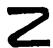
\includegraphics[keepaspectratio]{images/part001_8f5d44fd.jpg}}

\begin{enumerate}
\def\labelenumi{\arabic{enumi}.}
\setcounter{enumi}{4}
\tightlist
\item
  每一章的逻辑框架由该章的定义、公理和定理组成。这些是日后使用时主要需要记住的部分。较次要的结果以及那些容易由定理推出的结果被称为“命题”、“引理”、“推论”、“注记”等。初读时可以略去的那些内容以小号字体排印。对特别重要定理的评注偶尔以“附释”之名出现。
\end{enumerate}

为避免乏味的重复，有时引入仅在某一章或某一章的某一节内有效的记号或缩写是方便的（例如，在只讨论交换环的一章中，“环”一词总是指“交换环”）。这类约定总是被明确指出，一般出现在使用它的那一章的开头。

\begin{enumerate}
\def\labelenumi{\arabic{enumi}.}
\setcounter{enumi}{5}
\tightlist
\item
  正文中的某些段落旨在预先提醒读者以防严重的错误。这些段落在页边用符号
\end{enumerate}

Z（“危险弯道”）。

\begin{enumerate}
\def\labelenumi{\arabic{enumi}.}
\setcounter{enumi}{6}
\item
  习题的目的，既在于使读者能确信自己已消化正文，也在于使他注意到那些在正文中没有位置但仍有意义的结果。最难的习题带有符号 ¶。
\item
  一般地说，我们沿用通行的术语，除非看起来有充分理由偏离它。
\item
  我们特别注意始终使用严格正确的语言，同时不牺牲简单性。在正文中，我们尽可能指出语言的滥用；没有这类滥用，任何数学文本都有流于迂腐之虞，更不用说不可读。
\item
  由于正文原则上是对一个理论的教条式阐述，它一般不包含对文献的引用。书目式引用汇集于历史注记中，通常位于每章之末。这些注记在适当之处还包含关于该理论未解决问题的提示。
\end{enumerate}

跟随每个历史注记之后的参考书目，一般只包含那些在所论理论的发展过程中具有最重要意义的书籍和原始论文。它绝无自诩完备之意；特别是，仅用于确定优先权问题的引用几乎总是被略去。

至于习题，我们一般并不认为指出它们的来源是值得的，因为它们取自许多不同的来源（原始论文、教科书、习题集）。

11. 对本丛书某一部分的引用按如下方式给出：\par

\begin{enumerate}
\def\labelenumi{\alph{enumi})}
\item
  如果引用的是同一节中给出的定理、公理或定义，则按其编号引用。
\item
  如果它们出现在同一章的另一节中，则在引用中还给出该节。
\item
  如果它们出现在同一书的另一章中，则给出章和节。
\item
  如果它们出现在另一书中，则先按标题给出该书。
\end{enumerate}

结果摘要用字母 R 引用：例如《集合论》R 表示“《集合论》的结果摘要”。

\specialchapter{《数学原理》丛书目录}

\textbf{I. 集合论}\par

\begin{enumerate}
\def\labelenumi{\arabic{enumi}.}
\tightlist
\item
  形式数学的描述。2. 集合论。3. 有序集；基数；自然数。4. 结构。
\end{enumerate}

\textbf{II. 代数学}\par

\begin{enumerate}
\def\labelenumi{\arabic{enumi}.}
\tightlist
\item
  代数结构。2. 线性代数。3. 张量代数、外代数、对称代数。4. 多项式与有理分式。5. 域。6. 有序群与有序域。7. 主理想环上的模。8. 半单模与半单环。9. 半双线性型与二次型。
\end{enumerate}

\textbf{III. 一般拓扑学}\par

\begin{enumerate}
\def\labelenumi{\arabic{enumi}.}
\tightlist
\item
  拓扑结构。2. 一致结构。3. 拓扑群。4. 实数。5. 单参数群。6. 实数空间、仿射空间与射影空间。7. 加法群 \(\mathbf{R}^n\) 。8. 复数。9. 实数在一般拓扑中的使用。10. 函数空间。
\end{enumerate}

\textbf{IV. 一元实变量函数}\par

\begin{enumerate}
\def\labelenumi{\arabic{enumi}.}
\tightlist
\item
  导数。2. 原函数与积分。3. 初等函数。4. 微分方程。5. 函数的局部研究。6. 广义 Taylor 展开。Euler-Maclaurin 求和公式。7. Gamma 函数。辞典。
\end{enumerate}

\textbf{V. 拓扑向量空间}\par

\begin{enumerate}
\def\labelenumi{\arabic{enumi}.}
\tightlist
\item
  赋值域上的拓扑向量空间。2. 凸集与局部凸空间。3. 连续线性映射空间。4. 拓扑向量空间中的对偶性。5. Hilbert 空间：初等理论。辞典。
\end{enumerate}

\textbf{VI. 积分学}\par

\begin{enumerate}
\def\labelenumi{\arabic{enumi}.}
\tightlist
\item
  凸性不等式。2. Riesz 空间。3. 局部紧空间上的测度。4. 测度的扩张。L \(^{p}\) 空间。5. 测度的积分。6. 向量值积分。7. Haar 测度。8. 卷积与表示。9. Hausdorff 拓扑空间上的积分。
\end{enumerate}


\textbf{李群与李代数}\par

\begin{enumerate}
\def\labelenumi{\arabic{enumi}.}
\tightlist
\item
  李代数。2. 自由李代数。3. 李群。4. Coxeter 群与 Tits 系。5. 由反射生成的群。6. 根系。
\end{enumerate}

\textbf{交换代数}\par

\begin{enumerate}
\def\labelenumi{\arabic{enumi}.}
\tightlist
\item
  平坦模。2. 局部化。3. 分次、滤过与拓扑。4. 伴随素理想与准素分解。5. 整数。6. 赋值。7. 除子。
\end{enumerate}

\textbf{谱理论}\par

\begin{enumerate}
\def\labelenumi{\arabic{enumi}.}
\tightlist
\item
  赋范代数。2. 局部紧群。
\end{enumerate}

\textbf{微分流形与解析流形}\par

结果摘要。

\specialchapter{引言}

本书所处理的问题，是在代数数论以及（稍后的）代数几何的发展过程中产生的（参看历史注记）。从十九世纪起，这两个理论开始显示出显著的类似性；解决它们所提出的问题的尝试，导致分离出若干一般概念，其应用范围并不限于代数数环或代数函数环；而且，一如既往，以最一般的形式来考虑它们是有利的，这样才能看清它们的真正意义以及一项研究对另一项研究的影响。本书所处理的概念原则上可应用于所有交换环及其上的模；然而必须指出，实质性的结果常常只是在某些有限性假设（这些假设在经典情形总成立）之下才得到，例如假定模是有限生成的或环是 Noether 环。

开头几章的中心概念如下：

I. 局部化与整体化。例如，让我们从一个丢番图方程组出发：

\[
\mathrm{P} _ {i} (x _ {1}, \dots , x _ {m}) = 0 \quad (1 \leqslant i \leqslant n)\tag{*}
\]

其中 \(P_{i}\) 是整系数多项式，而要找的由有理整数组成的解 \((x_{i})\) 。可以先从寻找由有理数组成的解入手来接近这个问题，这相当于把 \(P_{i}\) 的系数视为 Z 的分式域 Q 的元素、并把所要的解取在 Q 中来考虑同一问题。第二步是考察：给定一个素数 p，是否存在分母不被 p 整除的有理数解（整数解显然满足这一条件）；在这种情形下，这相当于位于 Q 中由这种形式的有理数组成的子环 \(\mathbf{Z}_{(p)}\) 之内，该子环称为 Z 对应于素数 p 的局部环。显然，从 Z 到 Q 的过渡与从 Z 到 \(\mathbf{Z}_{(p)}\) 的过渡具有同一形式：在两种情形下，所允许的分母都不属于某个素理想（分别是理想 (0) 与理想 (p)）。“局部环”这一名称也出现在代数几何中，在那里这个概念以更自然的方式出现：例如，对于复系数单变量多项式的环 C{[}X{]}，对应于素理想 (X - \(\alpha\) ) 的局部环是在点 \(\alpha\) 处“正则”的（即在该点没有极点的）有理分式环。

每一个丢番图问题，更一般地，每一个关于 A-模（A 为交换环）的问题，都可以分解为两个辅助问题：先在与 A 的各个素理想 p 相应的局部环 \(A_{p}\) 中求解（“局部化”），然后问：能否由“局部化”问题对所有 p 都有解推出最初所提的问题有解（“从局部到整体的过渡”）。第二章专门研究这一双重过程，在那里还会看到，“局部化”并不只与素理想相关，而是有更广的适用范围。

\begin{enumerate}
\def\labelenumi{\Roman{enumi}.}
\setcounter{enumi}{1}
\tightlist
\item
  局部环的完备化。局部环 A 与域同样具有只有一个极大理想 m 的性质。利用这一事实，可以通过转向商环 A/m（因后者是域）在一定程度上把关于 A-模的问题变换为关于向量空间的类似问题。如果回到丢番图方程组 (*)，这一思想无非就是“模 p 约化”原理，即把方程变成模 p 的同余式，它从数论最早的工作起就自然地出现了。
\end{enumerate}

尽管如此，我们显然不能指望以这种方式得到原问题的完整结果，而且人们很快便认识到，为得到更精确的信息，必须不仅考虑模 m 的同余，还要考虑模 \(m^{n}\) 的“更高阶”同余，其中 n 为任意整数 n \textgreater{} 0。这样就会发现，n 越大，原问题在某种意义上就被“逼近”得越紧（例如在 A = Z 的情形，理由是一个 \(\neq 0\) 的整数不可能被一个给定素数 p 的所有幂 \(p^{n}\) 整除；因此只要 n 取得足够大，这个数就会在模 \(p^{n}\) 约化中显示出它的存在）。这一思想的数学转译，是在 A 上考虑一个环拓扑（参看《一般拓扑学》第三章 §6），其中诸 \(m^{n}\) 构成 0 的一个基本邻域系。但是，当我们例如已经解决了同余方程组

\[
\mathrm{P} _ {i} (x _ {1}, \dots , x _ {m}) \equiv 0 (\mathrm{mod.} p ^ {k}) \quad (1 \leqslant i \leqslant n)\tag{**}
\]

对每个整数 \(k > 0\) 成立时，仍然不能由此推出方程组 (*) 在局部环 \(\mathbf{Z}_{(p)}\) 中有解；上述假设可以解释为：(*) 在 \(\hat{\mathbf{Z}}_{(p)}\) （即拓扑环 \(\mathbf{Z}_{(p)}\) 的完备化）中有一个解。

这样削弱后的原问题，最终被变换为关于 A/m \(^{n}\) 型局部环的类似问题；这些环由于具有幂零根，
也比一般环更接近于域；在经典代数几何中，这对应于在给定点的邻域中对问题作“微分”式的研究。

第三章以一般的方式处理拓扑概念对局部环理论的这些应用。第六章研究其中一个特殊方面，它一方面适合于代数几何的更细致的研究，而尤其适合于代数数域的算术，在那里遇到的局部环（例如 \(\mathbf{Z}_{(p)}\) ）属于一类特别简单的环，即“赋值环”类；在赋值环中，可除性是主理想集合的一个全序（参看《代数学》第六章 §1）。

对从环 A 过渡到局部环 \(A_{p}\) 或完备化 \(\hat{A}\) 的研究，揭示了这两种运算的一个共同特征，即 A-模 \(A_{p}\) 与 \(\hat{A}\) 的平坦性；除其他作用外，它使得这类 A-模与任意 A-模的张量积的使用在某种程度上类似于向量空间张量积的使用，也就是说，无需一般情形下围绕其使用的种种预防措施。与这一概念相联系的性质也适用于非交换环上的模，它们是第一章的研究对象。

\begin{enumerate}
\def\labelenumi{\Roman{enumi}.}
\setcounter{enumi}{2}
\tightlist
\item
  整数与理想的分解。对代数数域中可除性的研究，从一开始就需要在这种域 K 中引入整数的概念，以推广域 Q 中有理整数的概念。“代数整数”这一概念的一般理论（如将看到的，它与非常严格的有限性条件相联系）在第五章中展开；它可以应用于所有交换环，并且不仅在算术中意义重大，在代数几何中、甚至在场 C 上的“解析空间”的现代理论中也意义重大。
\end{enumerate}

把经典算术扩张到代数整数环的主要障碍之一，长期以来在于有理整数分解为素因子的经典分解一般不能推广到这些环。为克服这一困难，必须创建理想的理论：这样，所寻求的唯一分解对理想成立，素理想的概念取代了素数的概念。此外，这一结果可以看作“从局部到整体的过渡”得以圆满实现的典型情形：对 \(x \in K\) ，知道 K 上所有“赋值”在 x 处的值，就能在相差一个可逆整数乘法的意义下确定 x。

在比代数整数环不那么简单的环中（甚至在多个未定元的多项式环中），这一结果不再成立。然而，可以用典范的方式使每个理想对应于一个完全确定的素理想集合：在代数几何中，如果考虑 \(K^{n}\)（K 为任意交换域）中由多项式方程组 \(P_{\alpha}=0\) 定义的子簇，则该子簇的不可约分支与由诸 \(P_{\alpha}\) 生成的理想所对应的素理想集合的极小元素一一对应。此外，（若限于 Noether 环）可以对每个理想给出一个比素理想之积的分解不那么精确的“分解”：这里乘积实际上被交集取代，而素理想的幂被与所论理想的伴随素理想相联系的“准素”理想所取代（但它们并不是素理想幂的直接推广）。与理想相伴随的素理想的引入及其性质的研究是第四章的主题；那里还证明了刚才提到的“准素分解”的存在性以及某些唯一性性质；但目前看来，这些分解在应用中通常只起辅助作用，本质性的概念是与理想相伴随的素理想。

在第七章中，我们将更详细地考察这样一些环：就分解为素理想之积而言，它们的性质最接近代数整数环的性质；除其他事项外，在这些环中可以引入“除子”的概念，它是这一分解的几何侧面，在代数几何中起重要作用。

最后，第八章及以后各章将处理在代数几何中比在算术中（在那里它们成为平凡的）更受关注的概念，特别是维数的概念。

有了这些概念，我们就到达了严格意义上的代数几何的边界，这是一条不断移动且难以划出的边界。因为，如果交换代数是使代数几何在其全部一般性中得到发展的本质工具，那么反过来（如上面已经看到的），几何语言对于表述交换代数的定理、并提示一种抽象代数中自然缺乏的直觉，显得非常方便；随着把代数几何的界限不断扩大得越来越多的趋势，代数的语言与几何的语言比以往任何时候都更加趋于融合。

第一章(*)

\chapter{平坦模}

除另有说明外，本章所考虑的环都假定具有单位元；所有环同态都假定把单位元映为单位元。环 A 的子环指包含 A 的单位元的子环。

如果 A 是环，M 是左 A-模，U（相应地 V）是 A（相应地 M）的加法子群，回顾一下，我们用 UV 或 U. V 表示由诸乘积 uv（其中 \(u \in U\) ， \(v \in V\) ）生成的 M 的加法子群（《代数学》第八章 §6 第 1 目）。若 a 是 A 的理想，我们写 \(a^{0} = A\) 。对任意集合 E，用 \(1_{E}\)（若不致混淆则简记为 1）表示 E 到自身的恒等映射。

回顾一下，模的公理蕴含：若 E 是环 A 上的左（相应地右）模，且 1 表示 A 的单位元，则对所有 \(x \in E\) 有 1.x = x（相应地 x.1 = x）（《代数学》第二章 §1 第 1 目）。若 E 和 F 是两个左（相应地右）A-模，回顾一下，我们用 \(\operatorname{Hom}_{\mathbf{A}}(\mathbf{E}, \mathbf{F})\)（或简记为 \(\operatorname{Hom}(\mathbf{E}, \mathbf{F})\) ）表示 E 到 F 的同态组成的加法群（出处同上，§1 第 2 目）。作为记号的滥用，我们常用 0 表示仅由其单位元组成的模。

\section{图与正合列}

\subsection{图}

例如，设 A, B, C, D, E 是五个集合，f 是从 A 到 B 的映射，g 是从 B 到 C 的映射，h 是从 D 到 E 的映射，u 是从 B 到 D 的映射，v 是从 C 到 E 的映射。为概括这样的情形，我们常使用图；例如，上述情形由下面的图概括（《集合论》第二章 §3 第 4 目）：

\begin{enumerate}
\def\labelenumi{(\arabic{enumi})}
\tightlist
\item
\end{enumerate}

\pandocbounded{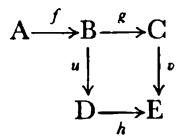
\includegraphics[keepaspectratio]{images/part001_a608eb63.jpg}}

在这样的图中，符号组 A \(\xrightarrow{f}\) B 以示意的方式表达 f 是从 A 到 B 的映射这一事实。当关于 f 不致有歧义时，我们省去字母 f 而简单地写 A \(\rightarrow\) B。

当 A, B, C, D, E 是群（相应地交换群）而 f, g, h, u, v 是群同态时，作为简称，称图 (1) 为群（相应地交换群）的图。

原则上，图不是数学对象，而只是为便于阅读论证而设计的一种图形。在实践中，图常被用作缩写符号，以避免一一列举所考虑的全部集合与映射；因此我们说“考虑图 (1)”，而不说“设 A, B, C, D, E 为五个集合……以及 v 是从 C 到 E 的映射”；例如见第 4 目中命题 2 的陈述。

\subsection{交换图}

例如，考虑下面的图：

\[
\begin{array}{c} \mathrm{A} \xrightarrow {f} \mathrm{B} \xrightarrow {g} \mathrm{C} \xrightarrow {h} \mathrm{D} \\ a \Big \downarrow \qquad b \Big \downarrow \qquad c \Big \downarrow \qquad d \Big \downarrow \\ \mathrm{A} ^ {\prime} \xrightarrow [ f ^ {\prime} ]{} \mathrm{B} ^ {\prime} \xrightarrow [ g ^ {\prime} ]{} \mathrm{C} ^ {\prime} \xrightarrow [ h ^ {\prime} ]{} \mathrm{D} ^ {\prime} \end{array}\tag{2}
\]

对每条由图中若干线段按箭头所示方向组成的路径，都对应着一个映射，它从第一条线段起点所表示的集合映到最后一条线段终点所表示的集合，即所经各线段所表示的映射的复合。对图的每个顶点，例如 B，按约定有一条化为 B 自身的路径，与之对应的是恒等映射 \(l_{B}\) 。

在 (2) 中，例如有三条从 A 出发到 C' 终止的路径；相应的映射为 \(c \circ g \circ f\) 、 \(g' \circ b \circ f\) 和 \(g' \circ f' \circ a\) 。称一个图为交换的，如果对图中每一对具有相同起点与终点的路径，相应的两个映射都相等；特别地，若一条路径的起点与终点重合，则相应的映射必须是恒等映射。

为使图 (2) 交换，必要且充分的是关系式

\[
f ^ {\prime} \circ a = b \circ f, \quad g ^ {\prime} \circ b = c \circ g, \quad h ^ {\prime} \circ f = d \circ h;\tag{3}
\]

成立；换言之，必要且充分的是 (2) 中所含的三个方形图都是交换的。因为关系式 (3) 蕴含 \(c \circ g \circ f = g' \circ b \circ f\) （由于 \(c \circ g = g' \circ b\) ），以及 \(g' \circ b \circ f = g' \circ f' \circ a\) （由于 \(b \circ f = f' \circ a\) ）；于是从 A 出发到 C' 终止的三条路径给出同一映射。类似地可以验证，从 A 出发到 D' 终止的四条路径（相应地，从 B 出发到 D' 终止的三条路径）给出同一映射。关系式 (3) 表示：从 A（相应地 B, C）出发到 B'（相应地 C', D'）终止的两条路径给出同一映射。(2) 的其他顶点对都不能用多于一条路径连接，因此图 (2) 是交换的。

在下文中，我们把其他类型图形的类似结果留给读者验证。

\subsection{正合列}

回顾下面的定义（《代数学》第二章 §1 第 4 目）：

定义 1. 设 A 是环，F, G, H 是三个右（相应地左）A-模，f 是 F 到 G 的同态，g 是 G 到 H 的同态。称有序偶 \((f, g)\) 为一个正合列，如果 \(\bar{g}^{-1}(0) = f(F)\) ，即如果 g 的核等于 f 的像。

图

\[
\mathrm{F} \xrightarrow {f} \mathrm{G} \xrightarrow {g} \mathrm{H}\tag{4}
\]

也称为一个正合列。

类似地，考虑一个由四个模和三个同态组成的图：

\[
\mathrm{E} \xrightarrow {f} \mathrm{F} \xrightarrow {g} \mathrm{G} \xrightarrow {h} \mathrm{H}.\tag{5}
\]

若图 \(E \xrightarrow{f} F \xrightarrow{g} G\) 是一个正合列，则称这个图在 F 处正合；若 \(F \xrightarrow{g} G \xrightarrow{h} H\) 是一个正合列，则称它在 G 处正合。若 (5) 在 F 和 G 处都正合，则称它是正合的，或也称它为一个正合列。任意多项的正合列可类似地定义。

回顾下面的结果（出处同上），其中 E, F, G 表示右（相应地左）

A-模，箭头表示同态，而 0 表示仅由其单位元组成的模：

\begin{enumerate}
\def\labelenumi{(\alph{enumi})}
\item
  说 \(0 \to \mathbf{E} \xrightarrow{f} \mathbf{F}\) 是一个正合列，等价于说 \(f\) 是单射。
\item
  说 \(\mathbf{E} \xrightarrow{f} \mathbf{F} \to 0\) 是一个正合列，等价于说 \(f\) 是满射。
\item
  说 \(0 \to \mathbf{E} \xrightarrow{f} \mathbf{F} \to 0\) 是一个正合列，等价于说 \(f\) 是双射，即 \(f\) 是 \(\mathbf{E}\) 到 \(\mathbf{F}\) 上的同构。
\item
  若 F 是 E 的子模，i 表示 F 到 E 中的典范单射，p 表示 E 到 E/F 上的典范满射，则图
\end{enumerate}

\[
0 \longrightarrow \mathrm{F} \stackrel {i} {\longrightarrow} \mathrm{E} \stackrel {p} {\longrightarrow} \mathrm{E} / \mathrm{F} \longrightarrow 0\tag{6}
\]

是一个正合列。

\begin{enumerate}
\def\labelenumi{(\alph{enumi})}
\setcounter{enumi}{4}
\tightlist
\item
  若 \(f: \mathbf{E} \to \mathbf{F}\) 是同态，则图
\end{enumerate}

\[
0 \longrightarrow \overline {{f}} ^ {- 1} (0) \stackrel {i} {\longrightarrow} \mathrm{E} \stackrel {f} {\longrightarrow} \mathrm{F} \stackrel {p} {\longrightarrow} \mathrm{F} / f (\mathrm{E}) \longrightarrow 0\tag{7}
\]

（其中 \(i\) 是 \(\overline{f}(0)\) 到 E 中的典范单射， \(p\) 是 \(\mathbf{F} / f(\mathbf{E})\) 的典范投影）是一个正合列。

\begin{enumerate}
\def\labelenumi{(\alph{enumi})}
\setcounter{enumi}{5}
\tightlist
\item
  为使图
\end{enumerate}

\[
\mathrm{E} \xrightarrow {f} \mathrm{F} \xrightarrow {g} \mathrm{G}\tag{8}
\]

成为一个正合列，必要且充分的是：存在模 S, T 以及同态 \(a: \mathrm{E} \to \mathrm{S}\) 、 \(b: \mathrm{S} \to \mathrm{F}\) 、 \(c: \mathrm{F} \to \mathrm{T}\) 和 \(d: \mathrm{T} \to \mathrm{G}\) ，使得 \(f = b \circ a\) 、 \(g = d \circ c\) ，且三个序列

\[
\begin{array}{c} \mathrm{E} \xrightarrow {a} \mathrm{S} \longrightarrow 0 \\ 0 \longrightarrow \mathrm{S} \xrightarrow {b} \mathrm{F} \xrightarrow {c} \mathrm{T} \longrightarrow 0 \\ 0 \longrightarrow \mathrm{T} \xrightarrow {d} \mathrm{G} \end{array}\tag{9}
\]

都是正合的。

最后回顾，若 \(f: \mathbf{E} \to \mathbf{F}\) 是 A-模同态，我们令 \(\operatorname{Ker}(f) = \bar{f}^{-1}(0)\) ， \(\operatorname{Im}(f) = f(\mathbf{E})\) ， \(\operatorname{Coim}(f) = \mathbf{E} / \bar{f}^{-1}(0)\) 和 \(\operatorname{Coker}(f) = \mathbf{F} / f(\mathbf{E})\) 。用这一记号，可以在 (9) 中取 \(\mathbf{S} = \operatorname{Im}(f) = \operatorname{Ker}(g)\) 和 \(\mathbf{T} = \operatorname{Im}(g)\) （典范同构于 \(\operatorname{Coker}(f)\) ）。

\subsection{蛇形图}

命题 1. 考虑交换群的一个交换图：

\[
\begin{array}{c c c} \mathrm{A} & \xrightarrow {u} & \mathrm{B} \\ a \Big \downarrow & & b \Big \downarrow \\ \mathrm{A} ^ {\prime} & \xrightarrow {} u ^ {\prime} & \mathrm{B} ^ {\prime} \end{array} \xrightarrow {v} \begin{array}{c c c} \mathrm{C} \\ c \Big \downarrow \\ \mathrm{C} ^ {\prime} \end{array}\tag{10}
\]

假设 (10) 的两行都是正合的。那么：

\begin{enumerate}
\def\labelenumi{(\roman{enumi})}
\tightlist
\item
  若 \(c\) 是单射，我们有
\end{enumerate}

\[
\operatorname{Im} (b) \cap \operatorname{Im} (u ^ {\prime}) = \operatorname{Im} (u ^ {\prime} \circ a) = \operatorname{Im} (b \circ u).\tag{11}
\]

\begin{enumerate}
\def\labelenumi{(\roman{enumi})}
\setcounter{enumi}{1}
\tightlist
\item
  若 \(a\) 是满射，我们有
\end{enumerate}

\[
\operatorname{Ker} (b) \dot {+} \operatorname{Im} (u) = \operatorname{Ker} (v ^ {\prime} \circ b) = \operatorname{Ker} (c \circ v).\tag{12}
\]

我们证明 (i)。显然

\[
\operatorname{Im} (u ^ {\prime} \circ a) = \operatorname{Im} (b \circ u) \subset \operatorname{Im} (b) \cap \operatorname{Im} (u ^ {\prime}).
\]

反之，设 \(x \in \operatorname{Im}(b) \cap \operatorname{Im}(u')\) 。存在 \(y \in B\) 使得 \(x = b(y)\) 。由于 \(v' \circ u' = 0\) ，我们有 \(0 = v'(x) = v'(b(y)) = c(v(y))\) ，由此得 \(v(y) = 0\) （因 \(c\) 是单射）。由于 \((u, v)\) 是正合列，存在 \(z \in A\) 使得 \(y = u(z)\) ，从而 \(x = b(u(z))\) 。

我们证明 (ii)。由于 \(v \circ u = 0\) 且 \(v' \circ u' = 0\) ，显然

\[
\operatorname{Ker} (b) + \operatorname{Im} (u) \subset \operatorname{Ker} (v ^ {\prime} \circ b) = \operatorname{Ker} (c \circ v).
\]

反之，设 \(x \in \operatorname{Ker}(v' \circ b)\) 。则 \(b(x) \in \operatorname{Ker}(v')\) ，且存在 \(y' \in A'\) 使得 \(u'(y') = b(x)\) （因序列 \((u', v')\) 正合）。由于 \(a\) 是满射，存在 \(y \in A\) 使得 \(a(y) = y'\) ，从而 \(b(x) = u'(a(y)) = b(u(y))\) ；由此得 \(x - u(y) \in \operatorname{Ker}(b)\) ，这样就完成了证明。

引理 1. 考虑交换群的一个交换图：

\[
\begin{array}{c} \mathrm{A} \xrightarrow {u} \mathrm{B} \\ a \Big \downarrow \\ \mathrm{A} ^ {\prime} \xrightarrow [ u ^ {\prime} ]{} \mathrm{B} ^ {\prime} \end{array}\tag{13}
\]

则存在一个且仅一个同态 \(u_1 \colon \operatorname{Ker}(a) \to \operatorname{Ker}(b)\) ，以及一个且仅一个同态 \(u_2 \colon \operatorname{Coker}(a) \to \operatorname{Coker}(b)\) ，使得诸图

\begin{enumerate}
\def\labelenumi{(\arabic{enumi})}
\setcounter{enumi}{13}
\tightlist
\item
\end{enumerate}

和

\pandocbounded{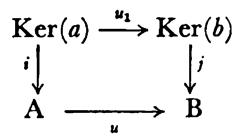
\includegraphics[keepaspectratio]{images/part001_d47c3bb2.jpg}}

\begin{enumerate}
\def\labelenumi{(\arabic{enumi})}
\setcounter{enumi}{14}
\tightlist
\item
\end{enumerate}

\pandocbounded{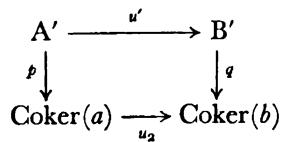
\includegraphics[keepaspectratio]{images/part001_9d56bddd.jpg}}

都是交换的，其中 \(i\) 和 \(j\) 表示典范单射， \(p\) 和 \(q\) 表示典范满射。

若 \(x \in \operatorname{Ker}(a)\) ，则 \(a(x) = 0\) 且 \(b(u(x)) = u'(a(x)) = 0\) ，因此 \(u(x) \in \operatorname{Ker}(b)\) ，于是 \(u_1\) 的存在性和唯一性是直接的。类似地，我们有 \(u'(a(A)) = b(u(A)) \subset b(B)\) ，然后取商， \(u'\) 给出一个同态 \(u_2\) ： \(\operatorname{Coker}(a) \to \operatorname{Coker}(b)\) ，它是使 (15) 交换的唯一的同态。

现在从交换群交换图 (10) 出发；由引理 1，与它对应有一个图

\begin{enumerate}
\def\labelenumi{(\arabic{enumi})}
\setcounter{enumi}{15}
\tightlist
\item
\end{enumerate}

\pandocbounded{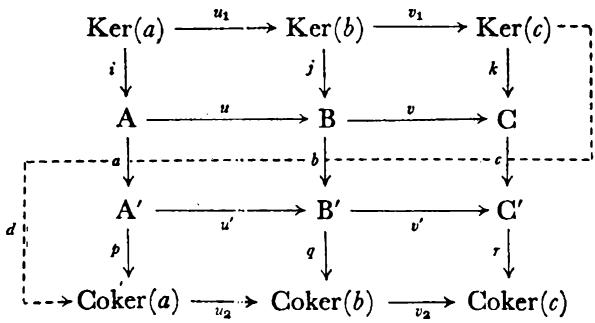
\includegraphics[keepaspectratio]{images/part001_af6ee28a.jpg}}

其中 \(i, j, k\) 是典范单射， \(p, q, r\) 是典范满射，而 \(u_{1}, u_{2}\) （相应地 \(v_{1}, v_{2}\) ）是由引理 1 典范地伴随于 \(u, u'\) （相应地 \(v, v'\) ）的同态。立即可验证这个图是交换的。

命题 2. 假设在交换图 (10) 中，序列 \((u, v)\) 和 \((u', v')\) 都是正合的。那么：

\begin{enumerate}
\def\labelenumi{(\roman{enumi})}
\item
  \(v_{1} \circ u_{1} = 0\) ；若 \(u'\) 是单射，则序列 \((u_{1}, v_{1})\) 正合。
\item
  \(v_{2} \circ u_{2} = 0\) ；若 \(v\) 是满射，则序列 \((u_{2}, v_{2})\) 正合。
\item
  假设 \(u'\) 是单射且 \(v\) 是满射。则存在一个且仅一个同态 \(d: \operatorname{Ker}(c) \to \operatorname{Coker}(a)\) ，它具有下列性质：若 \(x \in \operatorname{Ker}(c)\) ， \(y \in B\) 和 \(t' \in A'\) 满足关系 \(v(y) = k(x)\) 和 \(u'(t') = b(y)\) ，则 \(d(x) = p(t')\) 。此外，序列
\end{enumerate}

\[
(*) \quad \operatorname{Ker} (a) \xrightarrow {u _ {1}} \operatorname{Ker} (b) \xrightarrow {v _ {1}} \operatorname{Ker} (c) \xrightarrow {d}
\]

\[
\operatorname{Coker} (a) \xrightarrow {u _ {2}} \operatorname{Coker} (b) \xrightarrow {v _ {2}} \operatorname{Coker} (c)
\]

是正合的。

我们证明 (i)。由于 \(u_{1}\) 和 \(v_{1}\) 分别与 \(u\) 和 \(v\) 在 \(\operatorname{Ker}(a)\) 和 \(\operatorname{Ker}(b)\) 上的限制有相同的图，我们有 \(v_{1} \circ u_{1} = 0\) 。于是

\[
\operatorname{Ker} (v _ {1}) = \operatorname{Ker} (b) \cap \operatorname{Ker} (v) = \operatorname{Ker} (b) \cap \operatorname{Im} (u) = \operatorname{Im} (j) \cap \operatorname{Im} (u).
\]

但是，由命题 1 (i)，有 \(\operatorname{Ker}(v_1) = \operatorname{Im}(j \circ u_1) = \operatorname{Im}(u_1)\) （若 \(u'\) 是单射）。

我们证明 (ii)。由于 \(u_{2}\) 和 \(v_{2}\) 是由 \(u\) 和 \(v\) 取商得到的，显然 \(v_{2} \circ u_{2} = 0\) 。设 \(v\) 是满射；由于 \(q\) 和 \(p\) 是满射，由诸假设和命题 1 (ii) 得

\[
\begin{array}{r l} \operatorname{Ker} (v _ {2}) & = q (\operatorname{Ker} (v _ {2} \circ q)) = q (\operatorname{Ker} (v ^ {\prime}) + \operatorname{Im} (b)) = q (\operatorname{Ker} (v ^ {\prime})) = q (\operatorname{Im} (u ^ {\prime})) \\ & = \operatorname{Im} (q \circ u ^ {\prime}) = \operatorname{Im} (u _ {2} \circ p) = \operatorname{Im} (u _ {2}). \end{array}
\]

最后证明 (iii)。对 \(x \in \operatorname{Ker}(c)\) ，存在 \(y \in B\) 使得 \(v(y) = k(x)\) （因 \(v\) 是满射）；此外 \(v'(b(y)) = c(k(x)) = 0\) ，因而存在唯一的 \(t' \in A'\) 使得 \(u'(t') = b(y)\) （因 \(u'\) 是单射）。我们现在证明，元素 \(p(t') \in \operatorname{Coker}(a)\) 不依赖于元素 \(y \in B\) （只要 \(v(y) = k(x)\) ）。因为若 \(y' \in B\) 是另一个满足 \(v(y') = k(x)\) 的元素，则 \(y' = y + u(z)\) ，其中 \(z \in A\) ；我们证明：若 \(t'' \in A'\) 满足 \(u'(t'') = b(y')\) ，则 \(t'' = t' + a(z)\) ；因为

\[
u ^ {\prime} \left(t ^ {\prime} + a (z)\right) = u ^ {\prime} \left(t ^ {\prime}\right) + u ^ {\prime} (a (z)) = b (y) + b (u (z)) = b (y + u (z)) = b \left(y ^ {\prime}\right).
\]

最后，由此得 \(p(t'') = p(t') + p(a(z)) = p(t')\) 。于是可以令 \(d(x) = p(t')\) ，映射 \(d: \operatorname{Ker}(c) \to \operatorname{Coker}(a)\) 就这样被定义了。现在若 \(x_1, x_2\) 是 \(\operatorname{Ker}(c)\) 的元素且 \(x = x_1 + x_2\) ，我们取 B 的元素 \(y_1, y_2\) ，使得 \(v(y_1) = k(x_1)\) 和 \(v(y_2) = k(x_2)\) ，并为 \(y \in B\) 选取元素 \(y_1 + y_2\) ；于是立即可得 \(d(x) = d(x_1) + d(x_2)\) ，因而 \(d\) 是一个同态。

设 \(x = v_{1}(x')\) ，其中 \(x' \in \operatorname{Ker}(b)\) ；于是取 \(y \in B\) 为元素 \(j(x')\) 。由于 \(b(j(x')) = 0\) ，由此得 \(d(x) = 0\) ，因此 \(d \circ v_{1} = 0\) 。反之，设 \(d(x) = 0\) 。在上面的记号下，我们有 \(t' = a(s)\) ，其中 \(s \in A\) 。这时我们有 \(b(y) = u'(t') = u'(a(s)) = b(u(s))\) ，即 \(b(y - u(s)) = 0\) 。因此元素 \(y - u(s)\) 具有 \(j(n)\) 的形式，其中 \(n \in \operatorname{Ker}(b)\) ，并且我们有 \(k(x) = v(y) = v(u(s) + j(n)) = v(j(n)) = k(v_1(n))\) ；由于 \(k\) 是单射， \(x = v_1(n)\) ，这就证明了序列 (*) 在 \(\operatorname{Ker}(c)\) 处正合。

最后，我们有（始终用同一记号）

\[
u _ {2} (d (x)) = u _ {2} \left(p \left(t ^ {\prime}\right)\right) = q \left(u ^ {\prime} \left(t ^ {\prime}\right)\right) = q (b (y)) = 0
\]

因而 \(u_2 \circ d = 0\) 。反之，设 Coker(a) 的一个元素 \(w = p(t')\) 满足 \(u_2(w) = u_2(p(t')) = 0\) （其中 \(t' \in A'\) ）。则 \(q(u'(t')) = 0\) ，因而 \(u'(t') = b(y)\) 对某个 \(y \in B\) 成立；由于 \(v'(u'(t')) = 0\) ，我们有 \(v'(b(y)) = 0\) ，从而 \(c(v(y)) = 0\) ，换句话说， \(v(y) = k(x)\) 对某个 \(x \in \operatorname{Ker}(c)\) 成立，且按定义 \(w = d(x)\) ，这表明序列 (*) 在

Coker(a) 处正合。在 (i) 中已看到它在 \(\operatorname{Ker}(b)\) 处正合，在 (ii) 中它在 \(\operatorname{Coker}(b)\) 处正合，这就完成了 (iii) 的证明。

注记. 如果图 (10) 的群都是某个环 \(\Lambda\) 上的（例如右）模，且诸同态都是 \(\Lambda\) -模同态，则很快可以验证，命题 2 (iii) 中定义的同态 \(d\) 也是一个 \(\Lambda\) -模同态：若 \(x \in \operatorname{Ker}(c)\) 与 \(\alpha \in \Lambda\) ，且 \(y \in B\) 满足 \(v(y) = k(x)\) ，只需注意 \(v(y\alpha) = k(x\alpha)\) 。

推论 1. 假设图 (10) 是交换的且两行都正合。那么：

\begin{enumerate}
\def\labelenumi{(\roman{enumi})}
\item
  若 \(u'\) , \(a\) 和 \(c\) 都是单射，则 \(b\) 是单射。
\item
  若 \(v, a\) 和 \(c\) 都是满射，则 \(b\) 是满射。
\end{enumerate}

断言 (i) 是命题 2 的断言 (i) 的推论：因为 \(\operatorname{Ker}(a) = 0\) 且 \(\operatorname{Ker}(c) = 0\) ，所以 \(\operatorname{Ker}(b) = 0\) 。

断言 (ii) 是命题 2 的断言 (ii) 的推论：因为 \(\operatorname{Coker}(a) = 0\) 且 \(\operatorname{Coker}(c) = 0\) ，所以 \(\operatorname{Coker}(b) = 0\) 。

推论 2. 假设图 (10) 是交换的且两行都正合。在这些条件下：

\begin{enumerate}
\def\labelenumi{(\roman{enumi})}
\item
  若 \(b\) 是单射且 \(a\) 和 \(v\) 是满射，则 \(c\) 是单射。
\item
  若 \(b\) 是满射且 \(c\) 和 \(u'\) 是单射，则 \(a\) 是满射。
\end{enumerate}

为证明 (i)，考虑图

\[
\begin{array}{c c c} u (\mathrm{A}) & \xrightarrow {w} \mathrm{B} & \xrightarrow {v} \mathrm{C} \\ a ^ {\prime} \Big \downarrow & b \Big \downarrow & c \Big \downarrow \\ u ^ {\prime} (\mathrm{A} ^ {\prime}) & \xrightarrow [ w ^ {\prime} ]{} \mathrm{B} ^ {\prime} & \xrightarrow [ v ^ {\prime} ]{} \mathrm{C} ^ {\prime} \end{array}
\]

其中 \(a'\) 是与 b 在 \(u(\mathbf{A})\) 上的限制有相同图的映射，而 w 和 \(w'\) 是典范单射；显然这个图是交换的且它的行是正合的。此外 \(w'\) 是单射，且由假设 v 是满射；于是由命题 2 (iii)，我们有一个正合列

\[
0 = \operatorname{Ker} (b) \longrightarrow \operatorname{Ker} (c) \stackrel {d} {\longrightarrow} \operatorname{Coker} (a ^ {\prime}) = 0
\]

（因 \(b\) 是单射且 \(a'\) 是满射）；由此 \(\operatorname{Ker}(c) = 0\) 。

为证明 (ii)，考虑图

\[
\begin{array}{c} \mathrm{A} \xrightarrow {u} \mathrm{B} \xrightarrow {w} v (\mathrm{B}) \\ a ^ {\prime} \Biggl \downarrow \qquad \qquad b \Biggl \downarrow \qquad \qquad c ^ {\prime} \Biggl \downarrow \\ \mathrm{A} ^ {\prime} \xrightarrow [ w ^ {\prime} ]{} \mathrm{B} ^ {\prime} \xrightarrow [ v ^ {\prime} ]{} v ^ {\prime} (\mathrm{B} ^ {\prime}) \end{array}
\]

其中这次 \(c'\) 是与 c 在 \(v(\mathbf{B})\) 上的限制有相同图的映射，而 \(w\) 和 \(w'\) 分别与 \(v\) 和 \(v'\) 有相同的图；这个图是交换的且它的行是正合的。此外 \(w\) 是满射，且由假设 \(u'\) 是单射；于是由命题 2 (iii)，我们有一个正合列

\[
0 = \operatorname{Ker} (c ^ {\prime}) \xrightarrow {d} \operatorname{Coker} (a) \longrightarrow \operatorname{Coker} (b) = 0
\]

（因 \(b\) 是满射且 \(c'\) 是单射）；由此 Coker \((a) = 0\) 。

\section{平坦模}

\subsection{张量积的复习}

设 A 是环，E 是右 A-模，M 是左 A-模。在《代数学》第二章 §3 第 1 目中我们定义了张量积 \(\mathbf{E} \otimes_{\mathbf{A}} \mathbf{M}\) ，它是一个 \(\mathbf{Z}\) -模。若 \(\mathbf{E}'\) （相应地 \(\mathbf{M}'\) ）是右（相应地左）A-模，而 \(u: \mathbf{E} \to \mathbf{E}'\) （相应地 \(v: \mathbf{M} \to \mathbf{M}'\) ）是同态，我们也（出处同上，第 2 目）定义了一个 \(\mathbf{Z}\) -同态

\[
\boldsymbol {u} \otimes v: \mathrm{E} \otimes_ {\mathrm{A}} \mathrm{M} \rightarrow \mathrm{E} ^ {\prime} \otimes_ {\mathrm{A}} \mathrm{M} ^ {\prime}.
\]

引理 1. 设 \(\mathbf{M}' \xrightarrow{v} \mathbf{M} \xrightarrow{w} \mathbf{M}'' \to 0\) 是左 A-模的一个正合列，E 是一个右 A-模。则序列

\[
\mathrm{E} \otimes_ {\mathrm{A}} \mathrm{M} ^ {\prime} \xrightarrow {1 \otimes v} \mathrm{E} \otimes_ {\mathrm{A}} \mathrm{M} \xrightarrow {1 \otimes w} \mathrm{E} \otimes_ {\mathrm{A}} \mathrm{M} ^ {\prime \prime} \longrightarrow 0
\]

是交换群的正合列。

这就是《代数学》第二章 §3 第 6 目命题 5 的推论。

由此可知，对任意左 A-模同态 \(u: M \rightarrow N\) ，

\[
\mathrm{E} \otimes_ {\mathbf {A}} (\text { Coker } u)
\]

典范地等同于 \(\operatorname{Coker}(1_{E} \otimes u)\) ，这由把引理 1 应用于正合列

\[
\mathrm{M} \xrightarrow {u} \mathrm{N} \longrightarrow \text { Coker } u \longrightarrow 0.
\]

即得。在引理 1 的记号下，我们知道（出处同上），若 v 是单射，即若序列 \(0 \rightarrow M' \stackrel{v}{\rightarrow} M \stackrel{w}{\rightarrow} M'' \rightarrow 0\) 正合，并不能由此推出 \(1_{E} \otimes v\) 是单射，因此一般不能把 \(E \otimes_{A} M'\) 等同于 E \(\otimes_{\mathbf{A}}\) M 的一个子群。然而回顾（《代数学》第二章 §3 第 7 目命题 7 的推论 5）下面的结果：

引理 2. 若 \(v: \mathbf{M}' \to \mathbf{M}\) 是单射且 \(v(\mathbf{M}')\) 是 \(\mathbf{M}\) 的一个直因子，则同态 \(1_{\mathbf{E}} \otimes v\) 是单射，且它的像是 \(\mathbf{E} \otimes_{\mathbf{A}} \mathbf{M}\) 的一个直因子。

\subsection{M-平坦模}

定义 1. 设 A 是环，E 是右 A-模，M 是左 A-模。称 E 对 M 是平坦的（或 M-平坦的），如果对每个左 A-模 M' 和每个单同态 \(v: M' \to M\) ，同态 \(1_{E} \otimes v\) ： E \(\otimes_{A} M' \to E \otimes_{A} M\) 是单射。

对任意右 A-模 N，N-平坦左模的概念可类似地定义。说一个右 A-模 E 对一个左 A-模 M 是平坦的，等价于说 E 视为左 \(A^{0}\) -模（回顾 \(A^{0}\) 表示 A 的反环）时对右 \(A^{0}\) -模 M 是平坦的。

引理 3. 为使一个右 A-模 E 是 M-平坦的，必要且充分的是：对 M 的每个有限生成子模 M'，典范同态

\[
\mathbf {1} _ {\mathbf {E}} \otimes j: \mathbf {E} \otimes_ {\mathbf {A}} \mathbf {M} ^ {\prime} \rightarrow \mathbf {E} \otimes_ {\mathbf {A}} \mathbf {M}
\]

（j 为典范单射 \(\mathbf{M}'\to \mathbf{M}\) ）是单射的。

假设这一条件成立，并设 N 是 M 的任意子模。设在 \(E \otimes_{A} M\) 中，一个元素

\[
z = \sum_ {i} x _ {i} \otimes y _ {i} \in \mathbf {E} \otimes_ {\mathbf {A}} \mathbf {N} (x _ {i} \in \mathbf {E}, y _ {i} \in \mathbf {N})
\]

的典范像为零，并设 \(M'\) 是由诸 \(y_{i}\) 生成的 N 的有限生成子模；由于由假设复合映射 \(E \otimes_{A} M' \to E \otimes_{A} N \to E \otimes_{A} M\) 是单射的，把和 \(z' = \sum_{i} x_{i} \otimes y_{i}\) 视为 \(E \otimes_{A} M'\) 的元素时为零。由于 z 是 \(z'\) 的像，我们也有 z = 0，引理得证。

引理 4. 设 E 是右 A-模，M 是左 A-模，且 E 是 M-平坦的。若 N 是 M 的子模或商模，则 E 是 N-平坦的。

N 是子模的情形是容易的，因为若 \(N'\) 是 N 的子模，则复合同态

\[
\mathrm{E} \otimes_ {\mathrm{A}} \mathrm{N} ^ {\prime} \rightarrow \mathrm{E} \otimes_ {\mathrm{A}} \mathrm{N} \rightarrow \mathrm{E} \otimes_ {\mathrm{A}} \mathrm{M}
\]

是单射的，因此 \(\mathbf{E} \otimes_{\mathbf{A}} \mathbf{N}' \to \mathbf{E} \otimes_{\mathbf{A}} \mathbf{N}\) 也是单射的。于是设 \(\mathbf{N}\) 是 \(\mathbf{M}\) 的一个商模，即存在正合列 \(0 \to \mathbf{R} \xrightarrow{i} \mathbf{M} \xrightarrow{p} \mathbf{N} \to 0\) 。设 \(\mathbf{N}'\) 是 \(\mathbf{N}\) 的一个子模，并令 \(\mathbf{M}' = \bar{p}^{-1}(\mathbf{N}')\) 。用 \(i'\) 表示 \(\mathbf{R}\) 到 \(\mathbf{M}'\) 的、与 \(i, p'\) 中 i 有相同图的映射，以及 \(\mathbf{M}' \to \mathbf{N}'\) 的、与 \(p\) 在 \(\mathbf{M}'\) 上的限制有相同图的满射，用 \(r\) 表示 \(\mathbf{R}\) 到 \(\mathbf{R}\) 的恒等映射， \(m\) 表示典范单射 \(\mathbf{M}' \to \mathbf{M}\) ， \(n\) 表示典范单射 \(\mathbf{N}' \to \mathbf{N}\) 。图

\[
\begin{array}{c} 0 \longrightarrow \mathrm{R} \xrightarrow {i ^ {\prime}} \mathrm{M} ^ {\prime} \xrightarrow {p ^ {\prime}} \mathrm{N} ^ {\prime} \longrightarrow 0 \\ r \Biggl \downarrow \qquad m \Biggl \downarrow \qquad n \Biggl \downarrow \\ 0 \longrightarrow \mathrm{R} \xrightarrow [ i ]{} \mathrm{M} \xrightarrow [ p ]{} \mathrm{N} \longrightarrow 0 \end{array}
\]

是交换的且它的行是正合的。

为书写简单，我们令 \(\mathrm{T}(\mathbf{Q}) = \mathrm{E} \otimes_{\mathbf{A}} \mathbf{Q}\) （对每个左 A-模 \(\mathbf{Q}\) ），令 \(\mathrm{T}(v) = 1_{\mathbf{E}} \otimes v\) （对左 A-模的每个同态 \(v\) ）。图

\[
\begin{array}{l} \mathrm{T} (\mathrm{R}) \xrightarrow {\mathrm{T} (i ^ {\prime})} \mathrm{T} (\mathrm{M} ^ {\prime}) \xrightarrow {\mathrm{T} (p ^ {\prime})} \mathrm{T} (\mathrm{N} ^ {\prime}) \longrightarrow 0 \\ \mathrm{T} (r) \Bigg \downarrow \qquad \qquad \qquad \qquad \qquad \qquad \qquad \qquad \qquad \qquad \qquad \qquad \qquad \qquad \qquad \qquad \qquad \qquad \qquad \qquad \qquad \qquad \qquad \qquad \qquad \qquad \qquad \qquad \qquad \qquad \qquad \qquad \qquad \qquad \\ \mathrm{T} (\mathrm{R}) \xrightarrow [ \mathrm{T} (i) ]{} \mathrm{T} (\mathrm{M}) \xrightarrow [ \mathrm{T} (p) ]{} \mathrm{T} (\mathrm{N}) \longrightarrow 0 \end{array}
\]

是交换的，且由第 1 目引理 1，它的行是正合的。此外，由于 E 是 M-平坦的，同态 T(m) 是单射。由于 T(r) 和 T(p') 是满射，由 §1 第 4 目命题 2 的推论 2 得 T(n) 是单射，这就证明了引理。

引理 5. 设 \((\mathbf{M}_{\iota})_{\iota \in \mathbf{I}}\) 是一族左 A-模， \(\mathbf{M} = \bigoplus_{\iota \in \mathbf{I}} \mathbf{M}_{\iota}\) 是它们的直和，E 是一个右 A-模。若对所有 \(\iota \in \mathbf{I}\) ， E 对 \(\mathbf{M}_{\iota}\) 都是平坦的，则 E 对 M 是平坦的。

\begin{enumerate}
\def\labelenumi{(\alph{enumi})}
\tightlist
\item
  先设 \(I = \{1, 2\}\) ，并设 \(M'\) 是 \(M = M_{1} \oplus M_{2}\) 的子模，其中 \(M_{1}\) 和 \(M_{2}\) 典范地等同于 M 的子模。用 \(M_{1}'\) 表示交 \(M' \cap M_{1}\) ，用 \(M_{2}'\) 表示 \(M'\) 在 \(M_{2}\) 中、经 M 到 \(M_{2}\) 上的典范投影 p 之下的像。我们有一个图
\end{enumerate}

\[
\begin{array}{c} 0 \longrightarrow \mathrm{M} _ {1} ^ {\prime} \xrightarrow {i ^ {\prime}} \mathrm{M} ^ {\prime} \xrightarrow {p ^ {\prime}} \mathrm{M} _ {2} ^ {\prime} \longrightarrow 0 \\ v _ {1} \Biggl \downarrow \qquad \qquad \qquad \qquad \qquad \qquad \qquad \qquad \qquad \qquad \qquad \qquad \qquad v _ {2} \Biggl \downarrow \\ 0 \longrightarrow \mathrm{M} _ {1} \xrightarrow [ i ]{} \mathrm{M} \xrightarrow [ p ]{} \mathrm{M} _ {2} \longrightarrow 0 \end{array}
\]

其中 \(v_{1}, v, v_{2}, i, i'\) 是典范单射，而 \(p'\) 是与 p 在 M' 上的限制有相同图的映射，它是满射。立即可验证这个图是交换的且它的行是正合的。以证明引理 4 时相同的含义使用 T(Q) 和 T(v) ，我们有一个交换图

\[
\begin{array}{c} \mathrm{T} (\mathrm{M} _ {1} ^ {\prime}) \xrightarrow {\mathrm{T} (i ^ {\prime})} \mathrm{T} (\mathrm{M} ^ {\prime}) \xrightarrow {\mathrm{T} (p ^ {\prime})} \mathrm{T} (\mathrm{M} _ {2} ^ {\prime}) \\ \mathrm{T} (v _ {1}) \Biggl \downarrow \qquad \qquad \qquad \qquad \qquad \qquad \qquad \qquad \qquad \qquad \qquad \qquad \qquad \qquad \qquad \qquad \qquad \qquad \qquad \qquad \qquad \qquad \qquad \qquad \qquad \qquad \qquad \qquad \qquad \qquad \qquad \qquad \qquad \qquad \\ \mathrm{T} (\mathrm{M} _ {1}) \xrightarrow [ \mathrm{T} (i) ]{} \mathrm{T} (\mathrm{M}) \xrightarrow [ \mathrm{T} (p) ]{} \mathrm{T} (\mathrm{M} _ {2}) \end{array}
\]

由第 1 目的引理 1，这个图的两行都是正合的；由于 E 对 \(M_{1}\) 和 \(M_{2}\) 是平坦的， \(T(v_{1})\) 和 \(T(v_{2})\) 是单射；此外，由第 1 目的引理 2， \(T(i)\) 是单射。于是 §1 第 4 目命题 2 的推论 2 表明 \(T(v)\) 是单射，因而 E 是 M-平坦的。

\begin{enumerate}
\def\labelenumi{(\alph{enumi})}
\setcounter{enumi}{1}
\item
  若 I 是有 \(n\) 个元素的有限集，则利用 (a) 对 \(n\) 作归纳即得引理。
\item
  在一般情形，设 \(\mathbf{M}'\) 是 \(\mathbf{M}\) 的一个有限生成子模。则存在一个有限子集 \(J\) ，它包含在指标集 \(I\) 中，使得 \(\mathbf{M}'\) 包含于直和 \(\mathbf{M}_J = \bigoplus_{i \in J} \mathbf{M}_i\) 。由 (b) ， \(E\) 对 \(\mathbf{M}_J\) 是平坦的；因此典范同态 \(\mathbf{E} \otimes_{\mathbf{A}} \mathbf{M}' \to \mathbf{E} \otimes_{\mathbf{A}} \mathbf{M}_J\) 是单射的。另一方面，由于 \(\mathbf{M}_J\) 是 \(\mathbf{M}\) 的一个直因子，典范同态 \(\mathbf{E} \otimes_{\mathbf{A}} \mathbf{M}_J \to \mathbf{E} \otimes_{\mathbf{A}} \mathbf{M}\) 是单射的（第 1 目，引理 2）。取其复合，即得 \(\mathbf{E} \otimes_{\mathbf{A}} \mathbf{M}_J \to \mathbf{E} \otimes_{\mathbf{A}} \mathbf{M}\) 是单射的，从而由引理 3 ， \(E\) 对 \(M\) 是平坦的。
\end{enumerate}

\subsection{平坦模}

命题 1. 设 E 是右 A-模。下列三个性质等价：

\begin{enumerate}
\def\labelenumi{(\alph{enumi})}
\item
  E 对 \(A_{s}\) 是平坦的（换句话说，对 A 的每个左理想 a，典范同态 \(E \otimes_{A} a \to E \otimes_{A} A_{s} = E\) 是单射的）。
\item
  E 对每个左 A-模 M 都是 M-平坦的。
\item
  对左 A-模与同态的每个正合列
\end{enumerate}

\[
\mathrm{M} ^ {\prime} \xrightarrow {v} \mathrm{M} \xrightarrow {w} \mathrm{M} ^ {\prime \prime}
\]

序列

\[
\mathrm{E} \otimes_ {\mathrm{A}} \mathrm{M} ^ {\prime} \xrightarrow {1 \otimes v} \mathrm{E} \otimes_ {\mathrm{A}} \mathrm{M} \xrightarrow {1 \otimes w} \mathrm{E} \otimes_ {\mathrm{A}} \mathrm{M} ^ {\prime \prime}
\]

是正合的。

(b) 蕴含 (a) 是直接的。反之，设 (a) 成立；由第 2 目引理 5，E 对每个自由左 A-模都是平坦的；由于每个左 A-模都同构于一个自由模的商（《代数学》第二章 §1 第 11 目命题 20），由第 2 目的引理 4 即得 E 对 M 是平坦的。

我们证明 (c) 蕴含 (b)。若 \(v \colon \mathbf{M}' \to \mathbf{M}\) 是单同态，则序列 \(0 \to \mathbf{M}' \xrightarrow{v} \mathbf{M}\) 正合；由 (c)，序列

\[
0 \rightarrow \mathrm{E} \otimes_ {\mathrm{A}} \mathrm{M} ^ {\prime} \xrightarrow {1 \otimes v} \mathrm{E} \otimes_ {\mathrm{A}} \mathrm{M}
\]

是正合的；这表明 \(1 \otimes v\) 是单射，换句话说，E 是 M-平坦的。

最后，蕴含关系 \((\mathbf{b}) \Rightarrow (\mathbf{c})\) 是下面更精确的引理的推论：

引理 6. 若 \(\mathbf{M}' \xrightarrow{v} \mathbf{M} \xrightarrow{w} \mathbf{M}''\) 是左 A-模的一个正合列，且 E 是 \(\mathbf{M}''\) -平坦的右 A-模，则序列

\[
\mathrm{E} \otimes_ {\mathrm{A}} \mathrm{M} ^ {\prime} \xrightarrow {1 \otimes v} \mathrm{E} \otimes_ {\mathrm{A}} \mathrm{M} \xrightarrow {1 \otimes w} \mathrm{E} \otimes_ {\mathrm{A}} \mathrm{M} ^ {\prime \prime}
\]

是正合的。

我们以证明第 2 目引理 4 时的同一含义使用记号 \(\mathrm{T}(\mathbf{Q})\) 和 \(\mathrm{T}(v)\) 。记 \(\mathbf{M}_1'' = w(\mathbf{M})\) ，用 \(i: \mathbf{M}_1'' \to \mathbf{M}''\) 表示典范单射，用 \(p\) 表示 \(\mathbf{M}\) 到 \(\mathbf{M}_1''\) 的与 \(w\) 有相同图的映射。序列 \(\mathbf{M}' \xrightarrow{v} \mathbf{M} \xrightarrow{p} \mathbf{M}_1'' \to 0\) 正合，且由第 1 目引理 1 得序列

\[
\mathrm{T} (\mathbf {M} ^ {\prime}) \xrightarrow {\mathrm{T} (v)} \mathrm{T} (\mathbf {M}) \xrightarrow {\mathrm{T} (p)} \mathrm{T} (\mathbf {M} _ {1} ^ {\prime \prime}) \longrightarrow 0
\]

是正合的。此外，由于 E 对 \(\mathbf{M}''\) 是平坦的，映射 \(\mathrm{T}(i): \mathrm{T}(\mathbf{M}_1'') \to \mathrm{T}(\mathbf{M}'')\) 是单射的，且由于 \(\mathrm{T}(i) \circ \mathrm{T}(p) = \mathrm{T}(w)\) ，序列

\[
\mathrm{T} (\mathbf {M} ^ {\prime}) \xrightarrow {\mathrm{T} (v)} \mathrm{T} (\mathbf {M}) \xrightarrow {\mathrm{T} (w)} \mathrm{T} (\mathbf {M} ^ {\prime \prime})
\]

是正合的。（§1，第 3 目。）

定义 2. 称右 A-模 E 为平坦的，如果它具有命题 1 的诸等价性质。

左 A-模的平坦性可类似地定义。说一个右 A-模 E 是平坦的，等价于说 E 视为左 A \(^{0}\) -模时是平坦的。

注记

\begin{enumerate}
\def\labelenumi{(\arabic{enumi})}
\item
  由第 2 目的引理 3，为使右 A-模 E 是平坦的，必要且充分的是：对 A 的每个有限生成左理想 a，典范映射 \(E \otimes_{A} a \to E\) （命题 1，其像为 Ea）是单射的。
\item
  设 E 是平坦右 A-模。若 M' 是左 A-模 M 的子模，则典范单射 \(E \otimes_{A} M' \to E \otimes_{A} M\) 使我们可以把 \(E \otimes_{A} M'\) 等同于 \(E \otimes_{A} M\) 的一个子群。在此条件下，设 N 是一个左 A-模， \(u: M \to N\) 是一个同态，K = Ker u，I = Im u。考虑正合列
\end{enumerate}

\[
0 \longrightarrow \mathrm{K} \longrightarrow \mathrm{M} \stackrel {u} {\longrightarrow} \mathrm{N}
\]

即可看出（命题 1）， \(\mathbf{E} \otimes_{\mathbf{A}} (\operatorname{Ker} u)\) 等同于 \(\operatorname{Ker}(1_{\mathbf{E}} \otimes u)\) 。另一方面，用 \(u'\) 表示满同态 \(\mathbf{M} \to \mathbf{I}\) ，它与 \(u\) 有相同的图，用 \(i\) 表示典范单射 \(\mathbf{I} \to \mathbf{N}\) ，则 \(1_{\mathbf{E}} \otimes u'\) 是满射的（第 1 目，引理 1），且 \(1_{\mathbf{E}} \otimes i\) 是单射的（因 \(\mathbf{E}\) 是平坦的）。由于

\[
\mathbf {1} _ {\mathbf {E}} \otimes \boldsymbol {u} = (\mathbf {1} _ {\mathbf {E}} \otimes i) \circ (\mathbf {1} _ {\mathbf {E}} \otimes u ^ {\prime}),
\]

\(E \otimes_{A} (Im u) \text{ 等同于 } Im(1_{E} \otimes u).\)

命题 2. (i) 设 \((\mathbf{E}_t)_{t \in I}\) 是一族右 A-模。为使 \(\mathbf{E} = \bigoplus_{t \in I} \mathbf{E}_t\) 是平坦的，必要且充分的是诸 \(\mathbf{E}_t\) 都是平坦的。

\begin{enumerate}
\def\labelenumi{(\roman{enumi})}
\setcounter{enumi}{1}
\tightlist
\item
  设 \(\mathbf{I}\) 是一个有序集， \((\mathrm{E}_{\alpha}, f_{\beta \alpha})\) 是右 A-模的一个正向系（《代数学》第二章 §6 第 2 目）。若诸 \(\mathrm{E}_{\alpha}\) 中的每一个都是平坦的，则 \(\mathbf{E} = \varinjlim \mathrm{E}_{\alpha}\) 是平坦的。
\end{enumerate}

设 \(M' \to M\) 是一个单射的左 A-模同态。

\begin{enumerate}
\def\labelenumi{(\roman{enumi})}
\tightlist
\item
  为使直和同态
\end{enumerate}

\[
\bigoplus_ {i \in I} \left(E _ {i} \otimes_ {A} M ^ {\prime}\right)\rightarrow \bigoplus_ {i \in I} \left(E _ {i} \otimes_ {A} M\right)
\]

是正合的，必要且充分的是诸同态 \(\mathbf{E}_{\iota} \otimes_{\mathbf{A}} \mathbf{M}' \to \mathbf{E}_{\iota} \otimes_{\mathbf{A}} \mathbf{M}\) 中的每一个都如此（《代数学》第二章 §1 第 6 目命题 7 的推论 1）；由于 \(\bigoplus_{\iota \in \mathbf{I}} (\mathbf{E}_{\iota} \otimes_{\mathbf{A}} \mathbf{M})\) 典范地等同于 \(\mathbf{E} \otimes_{\mathbf{A}} \mathbf{M}\) （《代数学》第二章 §3 第 7 目命题 7），这就证明了 (i)。

\begin{enumerate}
\def\labelenumi{(\roman{enumi})}
\setcounter{enumi}{1}
\tightlist
\item
  由假设，诸序列
\end{enumerate}

\[
0 \rightarrow \mathrm{E} _ {\alpha} \otimes_ {\mathrm{A}} \mathrm{M} ^ {\prime} \rightarrow \mathrm{E} _ {\alpha} \otimes_ {\mathrm{A}} \mathrm{M}
\]

都是正合的，因而序列

\[
0 \rightarrow \mathrm{E} \otimes_ {\mathrm{A}} \mathrm{M} ^ {\prime} \rightarrow \mathrm{E} \otimes_ {\mathrm{A}} \mathrm{M}
\]

也是正合的，因为取正向极限与张量积可交换（《代数学》第二章 §6 第 3 目命题 7），且保持正合性（出处同上，§6 第 2 目命题 3）。

\subsection{平坦模的例子}

\begin{enumerate}
\def\labelenumi{(\arabic{enumi})}
\item
  对任意环 A， \(A_{d}\) 显然是平坦 A-模（《代数学》第二章 §3 第 4 目命题 4）。于是由第 3 目命题 2 (i) 得：每个自由右 A-模，以及更一般地每个投射右 A-模（《代数学》第二章 §2 第 2 目），都是平坦 A-模。
\item
  若 A 是半单环（《代数学》第八章 §5 第 1 目定义 1），则每个右 A-模 E 都是半单的，因而是一些单模的直和；由于这些单模中的每一个都同构于 \(\mathbf{A}_d\) 的一个直因子（出处同上，§5 第 1 目命题 6），E 是投射的，因此由 (1) 是平坦的（参看习题 16）。
\end{enumerate}

*(3) 在第二、三章中，我们将详细研究平坦 A-模的两个重要例子：分式环 \(S^{-1}A\) 以及 \(\hat{A}\) （即 \(A\) 关于 \(\mathfrak{I}\) -进拓扑的 Hausdorff 完备化）。*

命题 3. 设 A 是环，E 是右 A-模。

\begin{enumerate}
\def\labelenumi{(\roman{enumi})}
\item
  设 E 是平坦的。对 A 的每个不是 0 的右除子(*) 的元素 a，关系 \(x \in \mathbf{E}\) 、 \(xa = 0\) 蕴含 \(x = 0\) 。
\item
  设 A 是一个整环，其中每个有限生成理想都是主理想（例如主理想整环（《代数学》第七章 §1 第 1 目））。则 E 是平坦的，必要且充分的是 E 是无挠的。
\end{enumerate}

我们证明 (i)。设 \(v: \mathbf{A}_s \to \mathbf{A}_s\) 是左 A-模同态 \(t \mapsto ta\) ；假设表明 \(v\) 是单射的。由于 E 是平坦的，同态 \(1_{\mathbf{E}} \otimes v: \mathbf{E} \otimes_{\mathbf{A}} \mathbf{A}_s \to \mathbf{E} \otimes_{\mathbf{A}} \mathbf{A}_s\) 也是单射的。当 \(\mathbf{E} \otimes_{\mathbf{A}} \mathbf{A}_s\) 典范地等同于 E 时， \(1_{\mathbf{E}} \otimes v\) 就成为 E 的自同态 \(x \mapsto xa\) 。于是关系 \(xa = 0\) 蕴含 \(x = 0\) 。

我们证明 (ii)。由 (i)，若 E 是平坦的，则 E 是无挠的。反之，设 E 是无挠 A-模；我们验证，对 A 的每个有限生成理想 a，典范同态 \(E \otimes_{A} a \to E\) 是单射的（第 3 目，注记 1）。若 \(a = (0)\) ，这一断言是显然的；否则，由假设 a = Aa，其中 \(a \in A\) ， \(a \neq 0\) ，而 \(t \mapsto ta\) 就是 A 到 a 上的一个同构 v；用 i 表示典范单射 \(a \to A\) ， \(i \circ v\) 就是 E 上比为 a 的位似，且由于假设 E 无挠，它是单射的。于是 \(1_{E} \otimes (i \circ v) = (1_{E} \otimes i) \circ (1_{E} \otimes v)\) ；由于 \(1_{E} \otimes v\) 是同构， \(1_{E} \otimes i\) 是单射的，这就完成了证明。

例. 把命题 3 应用于环 \(\mathbf{Z}\) ，可以看出 \(\mathbf{Q}\) 是平坦 \(\mathbf{Z}\) -模，但 \(\mathbf{Z}/n\mathbf{Z}\) （对 \(n \geqslant 2\) ）不是平坦 \(\mathbf{Z}\) -模。

\subsection{商模的平坦性}

命题 4. 设 E 是右 A-模。下列三个性质等价：

\begin{enumerate}
\def\labelenumi{(\alph{enumi})}
\item
  E 是平坦的。
\item
  对形如
\end{enumerate}

\[
0 \longrightarrow \mathrm{G} \stackrel {v} {\longrightarrow} \mathrm{H} \stackrel {w} {\longrightarrow} \mathrm{E} \longrightarrow 0\tag{1}
\]

的右 A-模的每个正合列以及每个左 A-模 F，序列

\[
0 \longrightarrow \mathrm{G} \otimes_ {\mathrm{A}} \mathrm{F} \xrightarrow {v \otimes 1} \mathrm{H} \otimes_ {\mathrm{A}} \mathrm{F} \xrightarrow {w \otimes 1} \mathrm{E} \otimes_ {\mathrm{A}} \mathrm{F} \longrightarrow 0\tag{2}
\]

是正合的。

\begin{enumerate}
\def\labelenumi{(\alph{enumi})}
\setcounter{enumi}{2}
\tightlist
\item
  存在一个正合列 (1)，其中 H 是平坦的，使得对每个形如 \(A_{s}/a\) 的左 A-模 F，序列 (2) 都正合，这里 a 是 A 的一个有限生成左理想。
\end{enumerate}

我们先证明 (a) 蕴含 (b)。左 A-模 F 同构于一个自由模的商（《代数学》第二章 §1 第 11 目命题 20）；换句话说，我们有正合列

\[
0 \longrightarrow \mathrm{R} \stackrel {i} {\longrightarrow} \mathrm{L} \stackrel {p} {\longrightarrow} \mathrm{F} \longrightarrow 0
\]

其中 L 是自由的。考虑图

\[
\begin{array}{c} \mathrm{G} \otimes \mathrm{R} \xrightarrow {v \otimes 1 _ {\mathrm{R}}} \mathrm{H} \otimes \mathrm{R} \xrightarrow {w \otimes 1 _ {\mathrm{R}}} \mathrm{E} \otimes \mathrm{R} \\ \downarrow_ {1 _ {\mathrm{G}} \otimes i} \\ \mathrm{G} \otimes \mathrm{L} \xrightarrow {v \otimes 1 _ {\mathrm{L}}} \mathrm{H} \otimes \mathrm{L} \xrightarrow {w \otimes 1 _ {\mathrm{L}}} \mathrm{E} \otimes \mathrm{L} \\ \downarrow_ {1 _ {\mathrm{G}} \otimes p} \\ \mathrm{G} \otimes \mathrm{F} \xrightarrow {v \otimes 1 _ {\mathrm{F}}} \mathrm{H} \otimes \mathrm{F} \end{array}\tag{3}
\]

立即可得这个图是交换的，且由第 1 目的引理 1，它的行与列都正合；此外，由于 \(\mathbf{1}_{\mathbf{G}} \otimes p\) 和 \(\mathbf{1}_{\mathbf{H}} \otimes p\) 是满射的（第 1 目，引理 1），我们有 \(\mathbf{G} \otimes \mathbf{F} = \operatorname{Coker}(\mathbf{1}_{\mathbf{G}} \otimes i)\) ，

\[
\mathbf {H} \otimes \mathbf {F} = \operatorname{Coker} (\mathbf {1} _ {\mathbf {H}} \otimes i);
\]

\(w \otimes l_{R}\) 是满射的（第 1 目，引理 1）；最后，由于 L 自由因而是平坦的， \(v \otimes l_{L}\) 是单射的。于是可以应用蛇形图（§1 第 4 目，命题 2 (iii)）证明存在正合列

\[
\operatorname{Ker} \left(\mathrm{l} _ {\mathrm{H}} \otimes i\right) \longrightarrow \operatorname{Ker} \left(\mathrm{l} _ {\mathrm{E}} \otimes i\right) \xrightarrow {d} \mathrm{G} \otimes \mathrm{F} \xrightarrow {v \otimes \mathrm{l} _ {\mathrm{F}}} \mathrm{H} \otimes \mathrm{F}.\tag{4}
\]

在此条件下，若 E 是平坦的，则 \(1_{E} \otimes i\) 是单射的，换句话说 \(\operatorname{Ker}(1_{\mathbf{E}} \otimes i) = 0\) ，而正合列 (4) 表明 \(v \otimes 1_{F}\) 是单射的，因此序列 (2) 是正合的（考虑到第 1 目的引理 1）。

由于 (b) 显然蕴含 (c)，剩下要证明 (c) 蕴含 (a)。在 \(\mathbf{R} = \mathfrak{a}\) 、 \(\mathbf{L} = \mathbf{A}_s\) 、 \(\mathbf{F} = \mathbf{A}_s / \mathfrak{a}\) 的情形考虑图 (3)，并应用正合列 (4)。由假设 \(v \otimes 1_{\mathbb{F}}\) 是单射的，因此 \(\operatorname{Im}(d) = 0\) ；此外，由于 H 是平坦的，我们有 \(\operatorname{Ker}(1_{\mathbb{H}} \otimes i) = 0\) ；于是序列 (4) 的正合性蕴含 \(\operatorname{Ker}(1_{\mathbb{E}} \otimes i) = 0\) ，换句话说， \(1_{\mathbb{E}} \otimes i\) 是单射的，这就证明了 E 是平坦的（第 3 目，注记 1）。

命题 5. 设 \(0 \to E' \xrightarrow{v} E \xrightarrow{w} E'' \to 0\) 是右 A-模的一个正合列。设 \(E''\) 是平坦的。则为使 \(E\) 是平坦的，必要且充分的是 \(E'\) 是平坦的。

设 \(u: F' \to F\) 是左 A-模的一个单同态。考虑图

\[
\begin{array}{c} \mathrm{E} ^ {\prime} \otimes \mathrm{F} ^ {\prime} \xrightarrow {v \otimes 1 _ {\mathrm{F} ^ {\prime}}} \mathrm{E} \otimes \mathrm{F} ^ {\prime} \xrightarrow {w \otimes 1 _ {\mathrm{F} ^ {\prime}}} \mathrm{E} ^ {\prime \prime} \otimes \mathrm{F} ^ {\prime} \\ 1 _ {\mathrm{E} ^ {\prime}} \otimes u \Bigg \downarrow \qquad \qquad \qquad \qquad \qquad \qquad \qquad \qquad \qquad \qquad \qquad \qquad \qquad \qquad \qquad \qquad \qquad \qquad \qquad \qquad \qquad \qquad \qquad \qquad \qquad \qquad \qquad \qquad \qquad \qquad \qquad \qquad \qquad \qquad \\ \mathrm{E} ^ {\prime} \otimes \mathrm{F} \xrightarrow [ v \otimes 1 _ {\mathrm{F}} ]{} \mathrm{E} \otimes \mathrm{F} \xrightarrow [ w \otimes 1 _ {\mathrm{F}} ]{} \mathrm{E} ^ {\prime \prime} \otimes \mathrm{F} \end{array}
\]

它是交换的且它的行是正合的（第 1 目，引理 1）。由于 \(\mathbf{E}''\) 是平坦的，

\(1_{\mathbf{E}^{\prime \prime}} \otimes u\) 是单射的；此外，命题 4 证明 \(v \otimes 1_{\mathbf{F}^{\prime}}\) 和 \(v \otimes 1_{\mathbf{F}}\) 都是单射的。在此条件下，若 E 是平坦的，则 \(1_{\mathbf{E}} \otimes u\) 是单射的，因而

\[
\left(1 _ {\mathbf {E}} \otimes u\right) \circ (v \otimes 1 _ {\mathbf {F} ^ {\prime}}) = (v \otimes 1 _ {\mathbf {F}}) \circ \left(1 _ {\mathbf {E} ^ {\prime}} \otimes u\right);
\]

也是单射的；由此得 \(\mathbf{1}_{\mathbf{E}'} \otimes u\) 是单射的，从而 \(\mathbf{E}'\) 是平坦的。反之，若 \(\mathbf{E}'\) 是平坦的，则 \(\mathbf{1}_{\mathbf{E}'} \otimes u\) 是单射的；于是由 §1 第 4 目命题 2 的推论 1 得 \(\mathbf{1}_{\mathbf{E}} \otimes u\) 是单射的，因此 \(\mathbf{E}\) 是平坦的。

\textbf{注记}\par

\begin{enumerate}
\def\labelenumi{(\arabic{enumi})}
\item
  E 和 \(E'\) 都平坦而 \(E''\) 不平坦是可能的，Z-模的例子 \(E = Z\) 、 \(E' = nZ\) 、 \(E'' = Z/nZ\) （ \(n \geqslant 2\) ）就表明了这一点。
\item
  平坦模的子模不一定是平坦模（习题 3）。
\end{enumerate}

\subsection{交的性质}

引理 7. 设 E 是右 A-模，F 是左 A-模， \(\mathbf{F}'\) 、 \(\mathbf{F}''\) 是 F 的两个子模，使得 \(\mathbf{F} = \mathbf{F}' + \mathbf{F}''\) 。则 \(\mathbf{E} \otimes \mathbf{F}'\) 和 \(\mathbf{E} \otimes \mathbf{F}''\) 在 \(\mathbf{E} \otimes \mathbf{F}\) 中的典范像的交等于 \(\mathbf{E} \otimes (\mathbf{F}' \cap \mathbf{F}'')\) 的典范像。

考虑图

\[
\begin{array}{c} 0 \longrightarrow \mathrm{F} ^ {\prime} \cap \mathrm{F} ^ {\prime \prime} \longrightarrow \mathrm{F} ^ {\prime} \longrightarrow \mathrm{F} ^ {\prime} / (\mathrm{F} ^ {\prime} \cap \mathrm{F} ^ {\prime \prime}) \longrightarrow 0 \\ \Biggl \downarrow \quad \Biggl \downarrow \quad \text {   j   } \\ 0 \longrightarrow \mathrm{F} ^ {\prime \prime} \longrightarrow \mathrm{F} ^ {\prime} + \mathrm{F} ^ {\prime \prime} \longrightarrow (\mathrm{F} ^ {\prime} + \mathrm{F} ^ {\prime \prime}) / \mathrm{F} ^ {\prime \prime} \longrightarrow 0 \end{array}
\]

其中未标明的箭头是典范单射和满射，j 是《代数学》第一章 §6 第 13 目定理 6 中定义的典范同构。这个图是交换的且它的行是正合的。我们（由于 \(F = F' + F''\) ）得到一个交换图

\[
\begin{array}{c} \mathbf {E} \otimes (\mathbf {F} ^ {\prime} \cap \mathbf {F} ^ {\prime \prime}) \longrightarrow \mathbf {E} \otimes \mathbf {F} ^ {\prime} \longrightarrow \mathbf {E} \otimes (\mathbf {F} ^ {\prime} / (\mathbf {F} ^ {\prime} \cap \mathbf {F} ^ {\prime \prime})) \\ \Biggl \downarrow \qquad \qquad \qquad \qquad \qquad \qquad \qquad \qquad \qquad \qquad \qquad \qquad \qquad 1 _ {\mathbf {E}} \otimes \mathbf {j} \\ \mathbf {E} \otimes \mathbf {F} ^ {\prime \prime} \longrightarrow \mathbf {E} \otimes \mathbf {F} \longrightarrow \mathbf {E} \otimes (\mathbf {F} / \mathbf {F} ^ {\prime \prime}) \end{array}
\]

这个图的行是正合的（第 1 目，引理 1），且 \(1_{E} \otimes j\) 是同构。于是我们的断言是 §1 第 4 目命题 1 (i) 的特殊情形（参看习题 5）。

命题 6. 设 E 是右 A-模，F 是左 A-模，且 E 对 F 是平坦的。对 F 的每个子模 \(\mathbf{F}'\) ，我们用 \(\phi(\mathbf{F}')\) 表示 \(\mathbf{E} \otimes \mathbf{F}'\) 在 \(\mathbf{E} \otimes \mathbf{F}'\) 到 \(\mathbf{E} \otimes \mathbf{F}\) 的典范映射（由第 2 目的定义 1，它是单射的）之下的像。则若 \(\mathbf{F}'\) 、 \(\mathbf{F}''\) 是 F 的两个子模，我们有

\[
\phi (\mathbf {F} ^ {\prime} \cap \mathbf {F} ^ {\prime \prime}) = \phi (\mathbf {F} ^ {\prime}) \cap \phi (\mathbf {F} ^ {\prime \prime}).
\]

由于 E 对 F 平坦， \(\phi(F' + F'')\) 等同于 \(E \otimes (F' + F'')\) ，而子模 \(\phi(F')\) 、 \(\phi(F'')\) 和 \(\phi(F' \cap F'')\) 分别等同于 \(E \otimes F'\) 、 \(E \otimes F''\) 和 \(E \otimes (F' \cap F'')\) 在 \(E \otimes (F' + F'')\) 中的典范像。于是命题 6 由引理 7 得出。

注记 1. 在命题 6 的假设下，通常把 \(\mathbf{E} \otimes \mathbf{F}'\) 等同于 \(\phi(\mathbf{F}')\) （对 \(\mathbf{F}'\) 是 \(\mathbf{F}\) 的每个子模），由此得到公式

\[
\mathrm{E} \otimes_ {\mathrm{A}} (\mathrm{F} ^ {\prime} \cap \mathrm{F} ^ {\prime \prime}) = (\mathrm{E} \otimes_ {\mathrm{A}} \mathrm{F} ^ {\prime}) \cap (\mathrm{E} \otimes_ {\mathrm{A}} \mathrm{F} ^ {\prime \prime}).
\]

命题 7. 设 E 是右 A-模，E‘ 是 E 的子模，F 是左 A-模，F’ 是 F 的子模。设 E/E‘ 或 F/F’ 是平坦的。则 \(E' \otimes F'\) 在 \(E \otimes F\) 中的典范像等于 \(E' \otimes F\) 和 \(E \otimes F'\) 在 \(E \otimes F\) 中的典范像的交。

例如设 \(E/E'\) 是平坦的，考虑图

\[
\begin{array}{c} \mathrm{E} ^ {\prime} \otimes \mathrm{F} ^ {\prime} \longrightarrow \mathrm{E} \otimes \mathrm{F} ^ {\prime} \longrightarrow (\mathrm{E} / \mathrm{E} ^ {\prime}) \otimes \mathrm{F} ^ {\prime} \\ \Biggl \downarrow \qquad \qquad \qquad \qquad \qquad \qquad \qquad \qquad \qquad \qquad \qquad \qquad \qquad u \Biggl \downarrow \\ \mathrm{E} ^ {\prime} \otimes \mathrm{F} \longrightarrow \mathrm{E} \otimes \mathrm{F} \longrightarrow (\mathrm{E} / \mathrm{E} ^ {\prime}) \otimes \mathrm{F} \end{array}
\]

其中箭头是典范同态。这个图是交换的且它的行是正合的（第 1 目，引理 1）。由于 E/E' 是平坦的，u 是单射的。于是我们的断言是 §1 第 4 目命题 1 (i) 的特殊情形。

推论. 设 E 是右 A-模，E' 是 E 的子模。

\begin{enumerate}
\def\labelenumi{(\roman{enumi})}
\tightlist
\item
  设 \(\mathbf{E} / \mathbf{E}'\) 是平坦的。则对 \(\mathfrak{a}\) 取 \(\mathbf{A}\) 的每个左理想，
\end{enumerate}

\[
\mathbf {E} ^ {\prime} \mathfrak {a} = \mathbf {E} ^ {\prime} \cap \mathbf {E} \mathfrak {a}.\tag{5}
\]

\begin{enumerate}
\def\labelenumi{(\roman{enumi})}
\setcounter{enumi}{1}
\item
  反之，设 E 是平坦的，且对 A 的每个有限生成左理想 a，关系式 (5) 成立。则 E/E' 是平坦的。
\item
  只需把命题应用于 \(\mathbf{F} = \mathbf{A}_s\) ， \(\mathbf{F}' = a\) 的情形。
\item
  为证明 \(E/E'\) 是平坦的，应用第 5 目命题 4 的判别法 (c)；这时需要证明序列
\end{enumerate}

\[
0 \rightarrow \mathrm{E} ^ {\prime} / \mathrm{E} ^ {\prime} a \rightarrow \mathrm{E} / \mathrm{E} a \rightarrow \mathrm{E} / (\mathrm{E} ^ {\prime} + \mathrm{E} a) \rightarrow 0
\]

对 A 的每个有限生成左理想 a 在 E'/E'a 处正合。而这正是关系式 (5) 所表达的。

注记 2. 如果只假设 \(\mathbf{E} / \mathbf{E}'\) 对 F 平坦或 \(\mathbf{F} / \mathbf{F}'\) 对 E 平坦，命题 7 的结论仍然成立。

\subsection{平坦模的张量积}

设 A、B 是两个环，E 是右 A-模，F 是 (A, B)-双模（《代数学》第二章 §1 第 14 目）。回顾（《代数学》第二章 §3 第 4 目）， \(E \otimes_{A} F\) 具有一个典范的右 B-模结构，对此结构

\[
(x \otimes y) b = x \otimes (y b) \quad \text {   for   } \quad x \in \mathrm{E}, y \in \mathrm{F}, b \in \mathrm{B}.
\]

命题 8. 设 A、B 是两个环，E 是右 A-模，F 是 (A, B)-双模。设 E 是平坦的，且 F 作为 B-模是平坦的。则 B-模 \(E \otimes_{A} F\) 是平坦的。

设 G 是左 B-模， \(G'\) 是 G 的子模。由于 F 作为右 B-模是平坦的，典范同态 \(F \otimes_{B} G' \to F \otimes_{B} G\) 是单射的。由于 E 是平坦的，典范同态

\[
\mathrm{E} \otimes_ {\mathbf {A}} (\mathrm{F} \otimes_ {\mathbf {B}} \mathrm{G} ^ {\prime}) \rightarrow \mathrm{E} \otimes_ {\mathbf {A}} (\mathrm{F} \otimes_ {\mathbf {B}} \mathrm{G})
\]

是单射的。由于 \(E \otimes_{A} (F \otimes_{B} G')\) 和 \(E \otimes_{A} (F \otimes_{B} G)\) 分别典范地等同于 \((E \otimes_{A} F) \otimes_{B} G'\) 和 \((E \otimes_{A} F) \otimes_{B} G\) （《代数学》第二章 §3 第 8 目命题 8），典范同态

\[
(\mathbf {E} \otimes_ {\mathbf {A}} \mathbf {F}) \otimes_ {\mathbf {B}} \mathbf {G} ^ {\prime} \rightarrow (\mathbf {E} \otimes_ {\mathbf {A}} \mathbf {F}) \otimes_ {\mathbf {B}} \mathbf {G}
\]

是单射的，这就证明了 \(E \otimes_{A} F\) 是一个平坦 B-模。

推论 1. 设 C 是交换环，E、F 是两个平坦 C-模。则 \(E \otimes_{C} F\) 是平坦 C-模。

F 是 (C, C)-双模，只需取 B = A = C 应用命题 8。

推论 2. 设 \(\rho\) 是环 A 到环 B 的同态。若 E 是平坦右 A-模，则通过把基环扩张到 B（《代数学》第二章 §5 第 1 目）得到的右 B-模 \(\rho^{*}(\mathrm{E}) = \mathrm{E}_{(\mathrm{B})}\) 是平坦的。

按定义 \(E_{(B)} = E \otimes_{A} B\) ，其中 B 经由 \(\rho\) 被视为 (A, B)-双模。由于右 B-模 \(B_{d}\) 是平坦的，只需应用命题 8。

推论 3. 设 R、S 是两个环， \(\phi: \mathbf{R} \to \mathbf{S}\) 是环同态。若 M 是平坦右 S-模，且 \(\phi_*(\mathbf{S}_d)\) 是平坦右 R-模，则 \(\phi_*(\mathbf{M})\) 是平坦右 R-模。

回顾 \(\phi_{*}(\mathbf{M})\) 是由 \(x.r = x.\phi (r)\) （对所有 \(x\in \mathbf{M}\) 和所有 \(r\in \mathbb{R}\) ）定义的右 R-模（《代数学》第二章 §1 第 13 目）。于是取 \(\mathrm{A} = \mathrm{S}\) 、 \(\mathrm{B} = \mathrm{R}\) 、 \(\mathrm{E} = \mathrm{M}\) 、 \(\mathrm{F} = \mathrm{S}\) 应用命题 8，其中 S 具有 \(\phi\) 所定义的 (S, R)-双模结构；这时右 R-模 M \(\otimes_{\mathbf{S}}\) S 恰好就是 \(\phi_{*}(\mathbf{M})\) 。

命题 9. 设 \((\mathbf{A}_{\alpha}, f_{\beta \alpha})\) 是环的一个正向系， \(\mathbf{A} = \varinjlim \mathbf{A}_{\alpha}\) 是它的正向极限， \((\mathbf{E}_{\alpha}, f_{\beta \alpha})\) 是以同一指标集为指标的一族右 \(\mathbf{A}_{\alpha}\) -模的正向系， \(\mathbf{E} = \varinjlim \mathbf{E}_{\alpha}\) 是它的正向极限，它是一个右 A-模（《代数学》第二章 §6 第 2 目）。若诸 \(\mathbf{E}_{\alpha}\) 中的每一个都是平坦 \(\mathbf{A}_{\alpha}\) -模，则 \(\mathbf{E}\) 是平坦 A-模。

设 \(E_{\alpha}^{\prime}=E_{\alpha}\otimes_{A_{\alpha}}A\) ，其中 A 被视为左 \(A_{\alpha}\) -模（经由典范同态 \(A_{\alpha}\to A\) ）；我们知道右 A-模 E 典范地同构于 \(\varinjlim E_{\alpha}^{\prime}\) （出处同上，命题 7 的推论 2）。由命题 8 的推论 2 得， \(E_{\alpha}^{\prime}\) 对所有 \(\alpha\) 都是平坦右 A-模，因此由第 3 目的命题 2，E 是平坦 A-模。

\subsection{有限表示模}

设 \(\mathbf{A}\) 是环。左（相应地右）A-模的一个正合列

\[
\mathrm{L} _ {1} \rightarrow \mathrm{L} _ {0} \rightarrow \mathrm{E} \rightarrow 0\tag{6}
\]

其中 \(L_{0}\) 和 \(L_{1}\) 是自由的，称为左（相应地右）A-模 E 的一个表示（或长度为 1 的表示）。

每个 A-模 E 都有一个表示。事实上我们知道（《代数学》第二章 §1 第 11 目命题 20），存在一个满同态 \(u \colon \mathbf{L}_0 \to \mathbf{E}\) ，其中 \(\mathbf{L}_0\) 是自由的；若 \(\mathbf{R}\) 是 \(u\) 的核，则类似地存在满同态 \(v \colon \mathbf{L}_1 \to \mathbf{R}\) ，其中 \(\mathbf{L}_1\) 是自由的。若把 \(v\) 视为 \(\mathbf{L}_1\) 到 \(\mathbf{L}_0\) 的同态，则序列 \(\mathbf{L}_1 \xrightarrow{v} \mathbf{L}_0 \xrightarrow{u} 0\) 按定义是正合的，由此即得我们的断言。

若 \(\rho: \mathbf{A} \to \mathbf{B}\) 是环同态，则 \(\mathbf{E}\) 的每个表示 (6) 都诱导 \(\mathbf{E}_{(\mathbf{B})} = \mathbf{E} \otimes_{\mathbf{A}} \mathbf{B}\) 的一个表示：

\[
\mathrm{L} _ {1} \otimes_ {\mathrm{A}} \mathrm{B} \rightarrow \mathrm{L} _ {0} \otimes_ {\mathrm{A}} \mathrm{B} \rightarrow \mathrm{E} \otimes_ {\mathrm{A}} \mathrm{B} \rightarrow 0\tag{7}
\]

这由第 1 目的引理 1 以及 \(\mathbf{L} \otimes_{\mathbf{A}} \mathbf{B}\) 在 \(\mathbf{L}\) 自由时是自由 B-模这一事实得出。

模 E 的表示 (6) 称为有限的，如果自由模 \(L_{0}\) 和 \(L_{1}\) 都有有限基。显然，若表示 (6) 有限，则表示 (7) 也有限。称 E 为有限表示 A-模，如果它有一个有限表示。

断言 (i) 由定义直接得出。若 A 是左 Noether 环，且存在满同态 \(u \colon \mathbf{L}_0 \to \mathbf{E}\) ，其中 \(\mathbf{L}_0\) 是有有限基的自由左 A-模，则 \(u\) 的核 R 是有限生成的（《代数学》第八章 §2 第 1 目命题 1 及第 3 目命题 7），因而存在满同态 \(v \colon \mathbf{L}_1 \to \mathbf{R}\) ，其中 \(\mathbf{L}_1\) 是自由的且有有限基，而正合列 \(\mathbf{L}_1 \xrightarrow{v} \mathbf{L}_0 \xrightarrow{u} \mathbf{E} \to 0\) 是 E 的一个有限表示；由此得 (ii)。

最后，设 E 是一个有限生成的投射模；则它是有限生成自由模 \(L_{0}\) 的一个直因子（《代数学》第二章 §2 第 2 目命题 4 的推论）；满同态 \(L_{0} \rightarrow E\) 的核 R 于是同构于 \(L_{0}\) 的一个商，因而是有限生成的，然后像 (ii) 那样完成证明。

引理 9. 设 A 是环，E 是有限表示 A-模。对每个正合列

\[
0 \longrightarrow \mathrm{F} \stackrel {j} {\longrightarrow} \mathrm{G} \stackrel {p} {\longrightarrow} \mathrm{E} \longrightarrow 0
\]

其中 G 是有限生成的，模 F 是有限生成的。

设 \(L_{1} \stackrel{r}{\rightarrow} L_{0} \stackrel{s}{\rightarrow} E \rightarrow 0\) 是一个有限表示；若 \((e_{i})\) 是 \(L_{0}\) 的一个基，则对每个 i 存在元素 \(g_{i} \in G\) 使得 \(p(g_{i}) = s(e_{i})\) ；于是同态 \(u: L_{0} \rightarrow G\) （它对所有 i 满足 \(u(e_{i}) = g_{i}\) ）满足 \(s = p \circ u\) 。由于 \(s \circ r = 0\) ，我们有 \(u(r(L_{1})) \subset \operatorname{Ker} p\) ，且由于 \(\operatorname{Ker} p\) 同构于 F，可以看出存在同态 \(v: L_{1} \rightarrow F\) 使得图

\[
\begin{array}{c} \mathrm{L} _ {1} \xrightarrow {r} \mathrm{L} _ {0} \xrightarrow {s} \mathrm{E} \longrightarrow 0 \\ v \Biggl \downarrow \qquad \qquad u \Biggl \downarrow \qquad \qquad 1 _ {\mathrm{E}} \Biggl \downarrow \\ \mathrm{F} \xrightarrow {} _ {j} \mathrm{G} \xrightarrow {} _ {p} \mathrm{E} \longrightarrow 0 \end{array}
\]

是交换的。由于 \(j\) 是单射而 \(s\) 是满射，我们可以应用蛇形图（§1 第 4 目，命题 4），换句话说，存在正合列

\[
0 = \operatorname{Ker} 1 _ {\mathrm{E}} \xrightarrow {d} \text { Coker } v \longrightarrow \text { Coker } u \longrightarrow \text { Coker } 1 _ {\mathrm{E}} = 0.
\]

这表明 Coker v 同构于 \(G/u(L_{0})\) ，后者由假设是有限生成的。此外我们有正合列

\[
0 \rightarrow v (\mathrm{L} _ {1}) \rightarrow \mathrm{F} \rightarrow \text { Coker } v \rightarrow 0
\]

且由于 \(v(\mathbf{L}_1)\) 和 Coker \(v\) 都是有限生成的，F 也是有限生成的（《代数学》第二章 §1 第 7 目命题 9 的推论 5）。

\subsection{同态模中基环的扩张}

设 A 和 B 是两个环，E 是右 A-模，F 是右 B-模，G 是 (B, A)-双模。回顾我们曾定义（《代数学》第二章 §4 第 2 目）一个典范 Z-模同态

\[
\nu \colon \mathbf {F} \otimes_ {\mathbf {B}} \operatorname{Hom} _ {\mathbf {A}} (\mathbf {E}, \mathbf {G}) \rightarrow \operatorname{Hom} _ {\mathbf {A}} (\mathbf {E}, \mathbf {F} \otimes_ {\mathbf {B}} \mathbf {G})\tag{8}
\]

它使得对所有 \(y \in \mathbf{F}\) 和 \(u \in \operatorname{Hom}_{\mathbf{A}}(\mathbf{E}, \mathbf{G})\) ， \(\nu(y \otimes u)\) 是 A-线性映射 \(x \mapsto y \otimes u(x)\) 。

命题 10. 设 A、B 是两个环，E 是右 A-模，F 是右 B-模，G 是 (B, A)-双模。设 F 是平坦的。则若 E 是有限生成的（相应地有限表示的），典范同态 (8) 是单射的（相应地双射的）。

把 A、B、F、G 视为固定，并对每个右 A-模 E 令

\[
\mathrm{T} (\mathrm{E}) = \mathrm{F} \otimes_ {\mathrm{B}} \operatorname{Hom} _ {\mathrm{A}} (\mathrm{E}, \mathrm{G}), \quad \mathrm{T} ^ {\prime} (\mathrm{E}) = \operatorname{Hom} _ {\mathrm{A}} (\mathrm{E}, \mathrm{F} \otimes_ {\mathrm{B}} \mathrm{G})
\]

且用 \(\nu_{\mathbf{E}}\) 表示同态 (8)；对每个右 A-模同态 \(\nu: \mathbf{E} \to \mathbf{E}'\) ，令 \(\mathrm{T}(v) = 1_{\mathbf{F}} \otimes \mathrm{Hom}(v, 1_{\mathbf{G}})\) 和 \(\mathrm{T}'(v) = \mathrm{Hom}(v, 1_{\mathbf{F}} \otimes 1_{\mathbf{G}})\) 。设 \(\mathrm{L}_1 \xrightarrow{v} \mathrm{L}_0 \xrightarrow{w} \mathrm{E} \to 0\) 是 E 的一个表示；我们假设自由模 \(\mathrm{L}_0\) （相应地自由模 \(\mathrm{L}_0\) 和 \(\mathrm{L}_1\) ）是有限生成的。图

\[
\begin{array}{c} 0 \longrightarrow \mathrm{T(E)} \xrightarrow {\mathrm{T(w)}} \mathrm {T(L_ {0})} \xrightarrow {\mathrm{T(v)}} \mathrm {T(L_ {1})} \\ v _ {\mathbf {E}} \Biggl \downarrow \qquad \qquad \qquad \qquad \qquad \qquad \nu_ {\mathrm {L_ {0}}} \Biggl \downarrow \qquad \qquad \qquad \nu_ {\mathrm {L_ {1}}} \Biggl \downarrow \\ 0 \longrightarrow \mathrm {T^ {\prime} (E)} \xrightarrow {\mathrm {T^ {\prime} (w)}} \mathrm {T^ {\prime} (L_ {0})} \xrightarrow {\mathrm {T^ {\prime} (v)}} \mathrm {T^ {\prime} (L_ {1})} \end{array}\tag{9}
\]

是交换的，且第二行是正合的（《代数学》第二章 §2 第 1 目定理 1）；此外，序列

\[
0 \rightarrow \operatorname{Hom} _ {\mathbf {A}} (\mathrm{E}, \mathrm{G}) \rightarrow \operatorname{Hom} _ {\mathbf {A}} (\mathrm{L} _ {0}, \mathrm{G}) \rightarrow \operatorname{Hom} _ {\mathbf {A}} (\mathrm{L} _ {1}, \mathrm{G})
\]

是正合的（出处同上），且由于 F 是平坦的，(9) 的第一行也是一个正合列（第 3 目，命题 1）。于是我们知道 \(\nu_{\mathrm{L}_0}\) （相应地 \(\nu_{\mathrm{L}_0}\) 和 \(\nu_{\mathrm{L}_1}\) ）是双射的（《代数学》第二章 §4 第 2 目命题 2）。若只假设 \(\nu_{\mathrm{L}_0}\) 是双射的，则由 (9) 得

\[
\nu_ {\mathbf {L} _ {0}} \circ \mathbf {T} (w) = \mathbf {T} ^ {\prime} (w) \circ \nu_ {\mathbf {E}}
\]

是单射的，因而 \(v_{E}\) 也是单射的。若假设 \(v_{L_{0}}\) 和 \(v_{L_{1}}\) 都是双射的，则由 §1 第 4 目命题 2 的推论 2 (ii) 得 \(v_{E}\) 是满射的，而由于我们刚看到 \(v_{E}\) 是单射的，它是双射的。

\subsection{基环的扩张：交换环情形}

现在设 A 是交换环，B 是环， \(\rho: \mathbf{A} \to \mathbf{B}\) 是环同态，使得 \(\rho(\mathbf{A})\) 包含于 B 的中心；换句话说， \(\rho\) 在 B 上定义一个

A-代数结构。对每个 A-模 E，右 B-模 \(\mathrm{E}_{(\mathbf{B})} = \mathrm{E} \otimes_{\mathbf{A}} \mathbf{B}\) 于是等同于 \(B \otimes_{A} E\) ，因为由假设， \(\rho_{*}(B_{s})\) 和 \(\rho_{*}(B_{d})\) 的 A-模结构相同。回顾对每对由 A-模组成的有序偶 (E, F)，我们定义了一个典范 B-同态

\[
\omega : \left(\operatorname{Hom} _ {\mathbf {A}} (\mathrm{E}, \mathrm{F})\right) _ {(\mathbf {B})} \rightarrow \operatorname{Hom} _ {\mathbf {B}} \left(\mathrm{E} _ {(\mathbf {B})}, \mathrm{F} _ {(\mathbf {B})}\right)\tag{10}
\]

它使得对所有 \(u \in \operatorname{Hom}_{\mathbf{A}}(\mathrm{E}, \mathrm{F})\) 有 \(\omega(u \otimes 1) = u \otimes 1_{\mathbf{B}}\) （《代数学》第二章 §5 第 3 目）。

命题 11. 设 A 是交换环，B 是环， \(\rho\) 是 A 到 B 的中心的同态，E 和 F 是两个 A-模。设 B 是平坦 A-模，且 E 是有限生成的（相应地有限表示的）。则典范同态 (10) 是单射的（相应地双射的）。

由于 \(\omega\) 是典范同构

\[
\operatorname{Hom} _ {\mathbf {A}} (\mathrm{E}, \mathbf {B} \otimes_ {\mathbf {A}} \mathrm{F}) \rightarrow \operatorname{Hom} _ {\mathbf {B}} (\mathrm{E} _ {(\mathbf {B})}, \mathrm{F} _ {(\mathbf {B})})
\]

与典范同态 (8)

\[
\nu \colon \mathbf {B} \otimes_ {\mathbf {A}} \operatorname{Hom} _ {\mathbf {A}} (\mathbf {E}, \mathbf {F}) \rightarrow \operatorname{Hom} _ {\mathbf {A}} (\mathbf {E}, \mathbf {B} \otimes_ {\mathbf {A}} \mathbf {F})
\]

（出处同上）的复合，该命题是第 9 目命题 10 的推论。

现在设 A 和 B 都是交换的，考虑三个 A-模 \(E_{1}\) 、 \(E_{2}\) 、 \(E_{3}\) 和一个 A-双线性映射 \(f: E_{1} \times E_{2} \to E_{3}\) 。则存在一个且仅一个 B-双线性映射 \(f_{B}: E_{1(B)} \times E_{2(B)} \to E_{3(B)}\) 使得

\[
f _ {\mathrm{B}} (1 \otimes x _ {1}, 1 \otimes x _ {2}) = 1 \otimes f (x _ {1}, x _ {2})
\]

对所有 \(x_{1} \in \mathbf{E}_{1}, x_{2} \in \mathbf{E}_{2}\) 成立（《代数学》第九章 §1 第 4 目命题 1）。

在下面的陈述中，我们将假设 B 是平坦 A-模，且对每个子模 \(E'\) （ \(E_{i}\) 的，i = 1, 2, 3），我们将典范地把 \(E'_{(B)}\) 与它在 \(E_{i(B)}\) 中的像等同（第 3 目，注记 2）。

命题 12. 设 A、B 是交换环， \(\rho\) 是 A 到 B 的同态，E \(_{1}\) 、 E \(_{2}\) 、 E \(_{3}\) 是三个 A-模， \(f\) : E \(_{1} \times\) E \(_{2} \to\) E \(_{3}\) 是一个 A-双线性映射，而

\[
f _ {\mathbf {B}} \colon \mathrm{E} _ {1 (\mathbf {B})} \times \mathrm{E} _ {2 (\mathbf {B})} \rightarrow \mathrm{E} _ {3 (\mathbf {B})}
\]

是它的扩张。考虑子模 \(\mathbf{F}_2\) （含于 \(\mathbf{E}_2\) ）与子模 \(\mathbf{F}_3\) （含于 \(\mathbf{E}_3\) ），并用 \(\mathbf{T}\) 表示 \(\mathbf{E}_1\) 中由那些 \(x_1 \in \mathbf{E}_1\) （它们满足 \(f(x_1, x_2) \in \mathbf{F}_3\) ，对所有 \(x_2 \in \mathbf{F}_2\) ）组成的子模。设 \(\mathbf{B}\) 是平坦 A-模，且 \(\mathbf{F}_2\) 是有限生成的。则 \(\mathbf{T}_{(\mathbf{B})}\) 是由那些 \(x_1' \in \mathbf{E}_{1(\mathbf{B})}\) （它们满足 \(f_{\mathbf{B}}(x_1', x_2') \in \mathbf{F}_{3(\mathbf{B})}\) ，对所有 \(x_2' \in \mathbf{F}_{2(\mathbf{B})}\) ）组成的集合。

设 \(p\) 是典范满射 \(\mathrm{E}_3 \to \mathrm{E}_3 / \mathrm{F}_3\) ；对每个 \(x_1 \in \mathrm{E}_1\) ，我们让它对应 A-线性映射 \(x_2 \mapsto p(f(x_1, x_2))\) （ \(\mathrm{F}_2\) 到 \(\mathrm{E}_3 / \mathrm{F}_3\) 的），记之为 \(g(x_{1})\) ；于是 g 是 \(E_{1}\) 到 \(\operatorname{Hom}_{\mathbf{A}}(\mathbf{F}_{2}, \mathbf{E}_{3}/\mathbf{F}_{3})\) 的一个 A-同态，且 g 的核恰好就是 T。由于 B 是平坦 A-模，我们有正合列

\[
0 \longrightarrow \mathrm{T} _ {(\mathbf {B})} \longrightarrow \mathrm{E} _ {1 (\mathbf {B})} \stackrel {1 \otimes g} {\longrightarrow} \left(\operatorname{Hom} _ {\mathbf {A}} \left(\mathrm{F} _ {2}, \mathrm{E} _ {3} / \mathrm{F} _ {3}\right)\right) _ {(\mathbf {B})}
\]

（第 3 目，命题 1）。由命题 11，典范同态

\[
\omega : \left(\operatorname{Hom} _ {\mathbf {A}} (\mathrm{F} _ {2}, \mathrm{E} _ {3} / \mathrm{F} _ {3})\right) _ {(\mathbf {B})} \rightarrow \operatorname{Hom} _ {\mathbf {B}} (\mathrm{F} _ {2 (\mathbf {B})}, \left(\mathrm{E} _ {3} / \mathrm{F} _ {3}\right) _ {(\mathbf {B})})
\]

是单射的。另一方面，由于 B 是平坦 A-模， \((\mathrm{E}_{3}/\mathrm{F}_{3})_{(\mathrm{B})}\) 典范地等同于 \(E_{3(\mathrm{B})}/F_{3(\mathrm{B})}\) ；取 \(\omega\) 与 \(1 \otimes g\) 的复合，我们得到一个同态 u，序列 \(^{1}\)

\[
0 \longrightarrow \mathrm{T} _ {(\mathrm{B})} \longrightarrow \mathrm{E} _ {1 (\mathrm{B})} \stackrel {u} {\longrightarrow} \operatorname{Hom} _ {\mathrm{B}} \left(\mathrm{F} _ {2 (\mathrm{B})}, \mathrm{E} _ {3 (\mathrm{B})} / \mathrm{F} _ {3 (\mathrm{B})}\right)
\]

是正合的。由定义立即可得， \(u(x_{1}^{\prime})\) （其中

\[
x _ {1} ^ {\prime} = 1 \otimes x _ {1} \in \mathrm{E} _ {1 (\mathbf {B})},
\]

）是这样的线性映射：它把每个 \(x_2' \in \mathrm{F}_{2(\mathbf{B})}\) 映到模 \(\mathrm{F}_{3(\mathbf{B})}\) 下的 \(f_{\mathbf{B}}(x_1', x_2')\) 的剩余类；由线性性，这对所有 \(x_1' \in \mathrm{E}_{1(\mathbf{B})}\) 也成立；由于 \(u\) 的核是 \(\mathrm{T}_{(\mathbf{B})}\) ，命题得证。

推论 1. 设 A、B 是两个交换环， \(\rho: \mathbf{A} \to \mathbf{B}\) 是同态，使得 B 是平坦 A-模，E 是有限表示 A-模。对 E 的每个有限生成子模 F， \(\mathrm{E}_{(\mathrm{B})}\) 的对偶中与 \(\mathrm{F}_{(\mathrm{B})}\) 正交的子模等于 \((\mathrm{F}')_{(\mathrm{B})}\) ，其中 \(\mathrm{F}'\) 是 E 的对偶 \(\mathrm{E}^*\) 中与 F 正交的子模。

由命题 11， \((\mathbf{E}^{*})_{(\mathbf{B})}\) 典范地同构于对偶 \((\mathbf{E}_{(\mathbf{B})})^{*}\) （即 \(\mathbf{E}_{(\mathbf{B})}\) 的对偶）。于是只需取 \(\mathbf{E}_1 = \mathbf{E}^*\) 、 \(\mathbf{E}_2 = \mathbf{E}\) 、 \(\mathbf{E}_3 = \mathbf{A}\) 、 \(\mathbf{F}_2 = \mathbf{F}\) 、 \(\mathbf{F}_3 = \{0\}\) ，并取 \(f\) 为 \(\mathbf{E}^{*} \times \mathbf{E}\) 上的典范双线性型，来应用命题 12。

推论 2. 设 A、B 是两个交换环， \(\rho: A \to B\) 是同态，使得 B 是平坦 A-模，E 是 A-模。则对 E 的每个有限生成子模 F， \(F_{(B)}\) 的零化理想是 B 的理想 aB，其中 a 是 F 在 A 中的零化理想。

只需取 \(\mathbf{E}_1 = \mathbf{A}\) 、 \(\mathbf{E}_2 = \mathbf{E}_3 = \mathbf{E}\) 、 \(\mathbf{F}_2 = \mathbf{F}\) 、 \(\mathbf{F}_3 = \{0\}\) 应用命题 12。

注记. 如果关于模 \(E_{t}\) 与双线性映射 f 都没有歧义，则有时用 \(F_{3}: F_{2}\) 表示命题 12 中记作 T 的模，并称它为 \(F_{2}\) 到 \(F_{3}\) 的迁移子。于是命题 12 的结论可读作

\[
\mathrm{F} _ {3 (\mathrm{B})}: \mathrm{F} _ {2 (\mathrm{B})} = \left(\mathrm{F} _ {3}: \mathrm{F} _ {2}\right) _ {(\mathrm{B})}.\tag{11}
\]

在诸 \(E_{i}\) 都等于环 A、f 是乘法且诸 \(F_{i}\) 为理想 \(a_{i}\) 的特殊情形，我们得到迁移子公式

\[
\mathbf {B} \left(a _ {3}: a _ {2}\right) = \mathbf {B} a _ {3}: \mathbf {B} a _ {2}\tag{12}
\]

它在 B 是平坦 A-模且 \(a_{2}\) 是有限生成理想时成立。
